%% Version 6.1, 1 September 2021

% This tex file can be compiled with
% tectonic templateV5.tex
% https://tectonic-typesetting.github.io
%
% Or simply with the Overleaf latexmkrc configuration: (included in the repo)
% https://www.overleaf.com/learn/how-to/How_does_Overleaf_compile_my_project%3F
%
% A latexindent.yml config file is also included for easier and more consistent
% formatting.

%%%%%%%%%%%%%%%%%%%%%%%%%%%%%%%%%%%%%%%%%%%%%%%%%%%%%%%%%%%%%%%%%%%%%%
% TemplateV6.1.tex --  LaTeX-based blank template for submissions to the
% American Meteorological Society
%
%%%%%%%%%%%%%%%%%%%%%%%%%%%%%%%%%%%%%%%%%%%%%%%%%%%%%%%%%%%%%%%%%%%%%
% PREAMBLE
%%%%%%%%%%%%%%%%%%%%%%%%%%%%%%%%%%%%%%%%%%%%%%%%%%%%%%%%%%%%%%%%%%%%%

%% Start with one of the following:
% 1.5-SPACED VERSION FOR SUBMISSION TO THE AMS
\documentclass{ametsocV6.1}

% TWO-COLUMN JOURNAL PAGE LAYOUT---FOR AUTHOR USE ONLY
% \documentclass[twocol]{ametsocV6.1}

%%%%%%%%%%%%%%%%%%%%%%%%%%%%%%
% FOR PRINTING
\usepackage[a4paper]{geometry}
% MY ADDITIONS
\usepackage{colortbl}
\usepackage{multirow}
\usepackage[separate-uncertainty=true]{siunitx}
\usepackage[version=4]{mhchem}
% \usepackage[acronym]{glossaries}
\usepackage[automake]{glossaries-extra}
% \setacronymstyle{long-short}
\setabbreviationstyle[acronym]{long-short}
\setabbreviationstyle{short-long}
\makeglossaries{}
\newacronym{agcm}{AGCM}{Atmosphere General Circulation Model}
\newacronym{aodm}{AODVISstdn}{``stratospheric aerosol optical depth 550 nm day night''}
\newacronym{aod}{AOD}{(stratospheric) aerosol optical depth}
\newacronym{aogcm}{AOGCM}{Atmosphere-Ocean General Circulation Model}
\newacronym{c2wmp}{C2W\(-\)}{CESM2(WACCM6) intermediate strength}
\newacronym{c2wm}{C2W\(\downarrow\)}{CESM2(WACCM6) small strength}
\newacronym{c2wsn}{C2WN\(\uparrow\)}{CESM2(WACCM6) large strength, high northern latitude}
\newacronym{c2ws}{C2W\(\uparrow\)}{CESM2(WACCM6) large strength}
\newacronym{c2w}{C2W}{CESM2(WACCM6) tropical}
\newacronym{cam5}{CAM5}{Community Atmosphere Model Version 5}
\newacronym{cam6}{CAM6}{Community Atmosphere Model Version 6}
\newacronym{cesm1}{CESM1}{Community Earth System Model Version 1}
\newacronym{cesm2}{CESM2}{Community Earth System Model Version 2}
\newacronym{cesm}{CESM}{Community Earth System Model}
\newacronym{cice}{CICE5}{CICE Version 5.1.2}
\newacronym{cime}{CIME}{Common Infrastructure for Modelling the Earth}
\newacronym{cism}{CISM2}{Community Ice Sheet Model Version 2.1}
\newacronym{clm}{CLM5}{Community Land Model Version 5}
\newacronym{ecs}{ECS}{equilibrium climate sensitivity}
\newacronym{erf}{ERF}{effective radiative forcing}
\newabbreviation{ob16}{OB16}{\citet{ottobliesner2016}}
\newacronym{esm}{ESM}{Earth System Model}
\newacronym{flnt}{FLNT}{``net longwave flux at the top of the model''}
\newacronym{fpp}{FPP}{Filtered Poisson Process}
\newacronym{fsnt}{FSNT}{``net solar flux at the top of the model''}
\newacronym{fsst}{\texttt{fSST1850}}{fixed sea-surface temperature}
\newacronym{irf}{IRF}{instantaneous radiative forcing}
\newacronym{lwcf}{LWCF}{``long wave cloud forcing''}
\newacronym{lw}{LW}{long wave}
\newacronym{mam3}{MAM3}{three mode version of the Modal Aerosol Module}
\newacronym{mam}{MAM}{Modal Aerosol Module}
\newacronym{marbl}{MARBL}{MARine Biogeochemistry Library}
\newacronym{ma}{MA}{middle atmosphere}
\newacronym{mosart}{MOSART}{MOdel for Scale Adaptive River Transport}
\newabbreviation{j05}{J05}{\citet{jones2005}}
\newabbreviation{g16}{G16}{\citet{gregory2016}}
\newabbreviation{m20}{M20}{\citet{marshall2020dataset}}
\newabbreviation{t10}{T10}{\citet{timmreck2010}}
\newabbreviation{n15}{N15}{\citet{niemeier2015}}
\newacronym{pop}{POP2}{Parallel Ocean Program Version 2}
\newacronym{qbo}{QBO}{quasi-biennial oscillation}
\newacronym{rf}{RF}{(effective) radiative forcing}
\newacronym{swcf}{SWCF}{``short wave cloud forcing''}
\newacronym{sw}{SW}{short wave}
\newacronym{tcrp}{TCRP}{transient climate response parameter}
\newacronym{toa}{TOA}{top-of-the-atmosphere}
\newacronym{trefht}{TREFHT}{``reference height temperature''}
\newacronym{waccm}{WACCM6}{Whole Atmosphere Community Climate Model Version 6}
\newacronym{ww3}{WW3}{Wave Watch Version 3}
\newacronym{ytt}{YTT}{Young Toba Tuff}

% Create some custom commands
\newcommand{\iso}[1][i]{{#1}njected \ce{SO2}}
\definecolor{LightGray}{gray}{0.9}
% The content of the URL must be on its own line. The compiler works fine both ways, but
% the syntax highlighting is messed up by it.
\urldef\fssturl\url{
1850_CAM60%WCCM_CLM50%BGC-CROP_CICE%PRES_DOCN%DOM_MOSART_CISM2%NOEVOLVE_SWAV_TEST
}
%%%%%%%%%%%%%%%%%%%%%%%%%%%%%%

%%%%%%%%%%%%%%%%%%%%%%%%%%%%%%%%

%%% To be entered by author:

%% May use \\ to break lines in title:

\title{
  Parameter Scan: Volcanic influence on climate across multiple magnitudes of injected
  \ce{SO2}
}

%% Enter authors' names and affiliations as you see in the examples below.
%
%% Use \correspondingauthor{} and \thanks{} (\thanks command to be used for affiliations footnotes,
%% such as current affiliation, additional affiliation, deceased, co-first authors, etc.)
%% immediately following the appropriate author.
%
%% Note that the \correspondingauthor{} command is NECESSARY.
%% The \thanks{} commands are OPTIONAL.
%
%% Enter affiliations within the \affiliation{} field. Use \aff{#} to indicate the affiliation letter at both the
%% affiliation and at each author's name. Use \\ to insert line breaks to place each affiliation on its own line.

%\authors{Author One,\aff{a}\correspondingauthor{Author One, email@email.com}
%Author Two,\aff{a}
%Author Three,\aff{b}
%Author Four,\aff{a}
%Author Five\thanks{Author Five's current affiliation: NCAR, Boulder, Colorado},\aff{c}
%Author Six,\aff{c}
%Author Seven,\aff{d}
% and Author Eight\aff{a,d}
%}
%
%\affiliation{\aff{a}{First Affiliation}\\
%\aff{b}{Second Affiliation}\\
%\aff{c}{Third Affiliation}\\
%\aff{d}{Fourth Affiliation}
%}

\authors{
  Eirik Rolland Enger,\aff{a}\correspondingauthor{Eirik Rolland Enger, eirik.r.enger@uit.no}
  Rune Graversen,\aff{a}
  Audun Theodorsen,\aff{a}
  and Maria Rugenstein\aff{b}
}

\affiliation{
  \aff{a}{UiT The Arctic University of Norway, Tromsø, Norway}\\
  \aff{b}{Colorado State University, Fort Collins, Colorado}
}

%%%%%%%%%%%%%%%%%%%%%%%%%%%%%%%%%%%%%%%%%%%%%%%%%%%%%%%%%%%%%%%%%%%%%
% ABSTRACT
%
% Enter your abstract here
% Abstracts should not exceed 250 words in length!
%

\abstract{%
  Large to super-volcano sized eruptions are simulated in the \gls{cesm2} climate model
  with the \gls{waccm} atmosphere. Ensembles containing four members are simulated, and
  the \gls{aod}, \gls{rf} and temperature anomaly from the eruptions are compared.
  Simulating a Pinatubo-like eruption yields results consistent with several previous
  studies with a slope of \(\sim \SI{-20}{\watt\metre^{-2}}\) per unit \gls{aod} for
  \gls{rf}. Larger eruptions, however, give a shallower slope indicative of a lower
  forcing efficiency. Moreover, a time-after-eruption dependence between \gls{aod} and
  \gls{rf} is found, where the \gls{rf} is relatively stronger than \gls{aod} the first
  year after the eruption (higher forcing efficiency), while later their ratio is
  roughly constant for a given eruption strength.
}

% NOTE: On efficiency: Pitari (Stratospheric ..) discuss this as global RF normalised to
% global optical thickness. Also M20.

\begin{document}

%% Necessary!
\maketitle{} \glsresetall{}

%%%%%%%%%%%%%%%%%%%%%%%%%%%%%%%%%%%%%%%%%%%%%%%%%%%%%%%%%%%%%%%%%%%%%
% SIGNIFICANCE STATEMENT/CAPSULE SUMMARY
%%%%%%%%%%%%%%%%%%%%%%%%%%%%%%%%%%%%%%%%%%%%%%%%%%%%%%%%%%%%%%%%%%%%%
%
% If you are including an optional significance statement for a journal article or a required capsule summary for BAMS
% (see www.ametsoc.org/ams/index.cfm/publications/authors/journal-and-bams-authors/formatting-and-manuscript-components for details),
% please apply the necessary command as shown below:
%
% Significance Statement (all journals except BAMS)
%
%\statement
%	 Enter significance statement here, no more than 120 words. See \url{www.ametsoc.org/index.cfm/ams/publications/author-information/significance-statements/} for details.
%
%% Capsule (BAMS only)
%%
%\capsule
%       Enter BAMS capsule here, no more than 30 words. See \url{www.ametsoc.org/index.cfm/ams/publications/author-information/formatting-and-manuscript-components/#capsule} for details.
%
%% * * If using twocol mode, you will need to use the commands "twocolsig" and "twocolcapsule" in place of "sig" and "capsule"
%%      to ensure that the text box correctly spans across both columns.
%

%%%%%%%%%%%%%%%%%%%%%%%%%%%%%%%%%%%%%%%%%%%%%%%%%%%%%%%%%%%%%%%%%%%%%
% MAIN BODY OF PAPER
%%%%%%%%%%%%%%%%%%%%%%%%%%%%%%%%%%%%%%%%%%%%%%%%%%%%%%%%%%%%%%%%%%%%%
%

%% In all cases, if there is only one entry of this type within
%% the higher level heading, use the star form:
%%
% \section{Section title}
% \subsection*{subsection}
% text...
% \section{Section title}

%vs

% \section{Section title}
% \subsection{subsection one}
% text...
% \subsection{subsection two}
% \section{Section title}

%%%
% \section{First primary heading}

% \subsection{First secondary heading}

% \subsubsection{First tertiary heading}

% \paragraph{First quaternary heading}

%%%%%%%%%%%%%%%%%%%%%%%%%%%%%%%%%%%%%%%%%%%%%%%%%%%%%%%%%%%%%%%%%%%%%
% TABLES---INSERT NEAR IN-TEXT DISCUSSION
%%%%%%%%%%%%%%%%%%%%%%%%%%%%%%%%%%%%%%%%%%%%%%%%%%%%%%%%%%%%%%%%%%%%%
%%  Enter tables near where they are discussed within the document.
%%  Please place tables before/after paragraphs, not within a paragraph.
%%
%
%\begin{table}[t]
%\caption{This is a sample table caption and table layout.  Enter as many tables as
%  necessary at the end of your manuscript. Table from Lorenz (1963).}\label{t1}
%\begin{center}
%\begin{tabular}{ccccrrcrc}
%\hline\hline
%$N$ & $X$ & $Y$ & $Z$\\
%\hline
% 0000 & 0000 & 0010 & 0000 \\
% 0005 & 0004 & 0012 & 0000 \\
% 0010 & 0009 & 0020 & 0000 \\
% 0015 & 0016 & 0036 & 0002 \\
% 0020 & 0030 & 0066 & 0007 \\
% 0025 & 0054 & 0115 & 0024 \\
%\hline
%\end{tabular}
%\end{center}
%\end{table}

%%%%%%%%%%%%%%%%%%%%%%%%%%%%%%%%%%%%%%%%%%%%%%%%%%%%%%%%%%%%%%%%%%%%%
% FIGURES---INSERT NEAR IN-TEXT DISCUSSION
%%%%%%%%%%%%%%%%%%%%%%%%%%%%%%%%%%%%%%%%%%%%%%%%%%%%%%%%%%%%%%%%%%%%%
%%  Enter figures near where they are discussed within the document.
%%  Please place figures before/after paragraphs, not within a paragraph.
% %
%
%\begin{figure}[t]
%  \noindent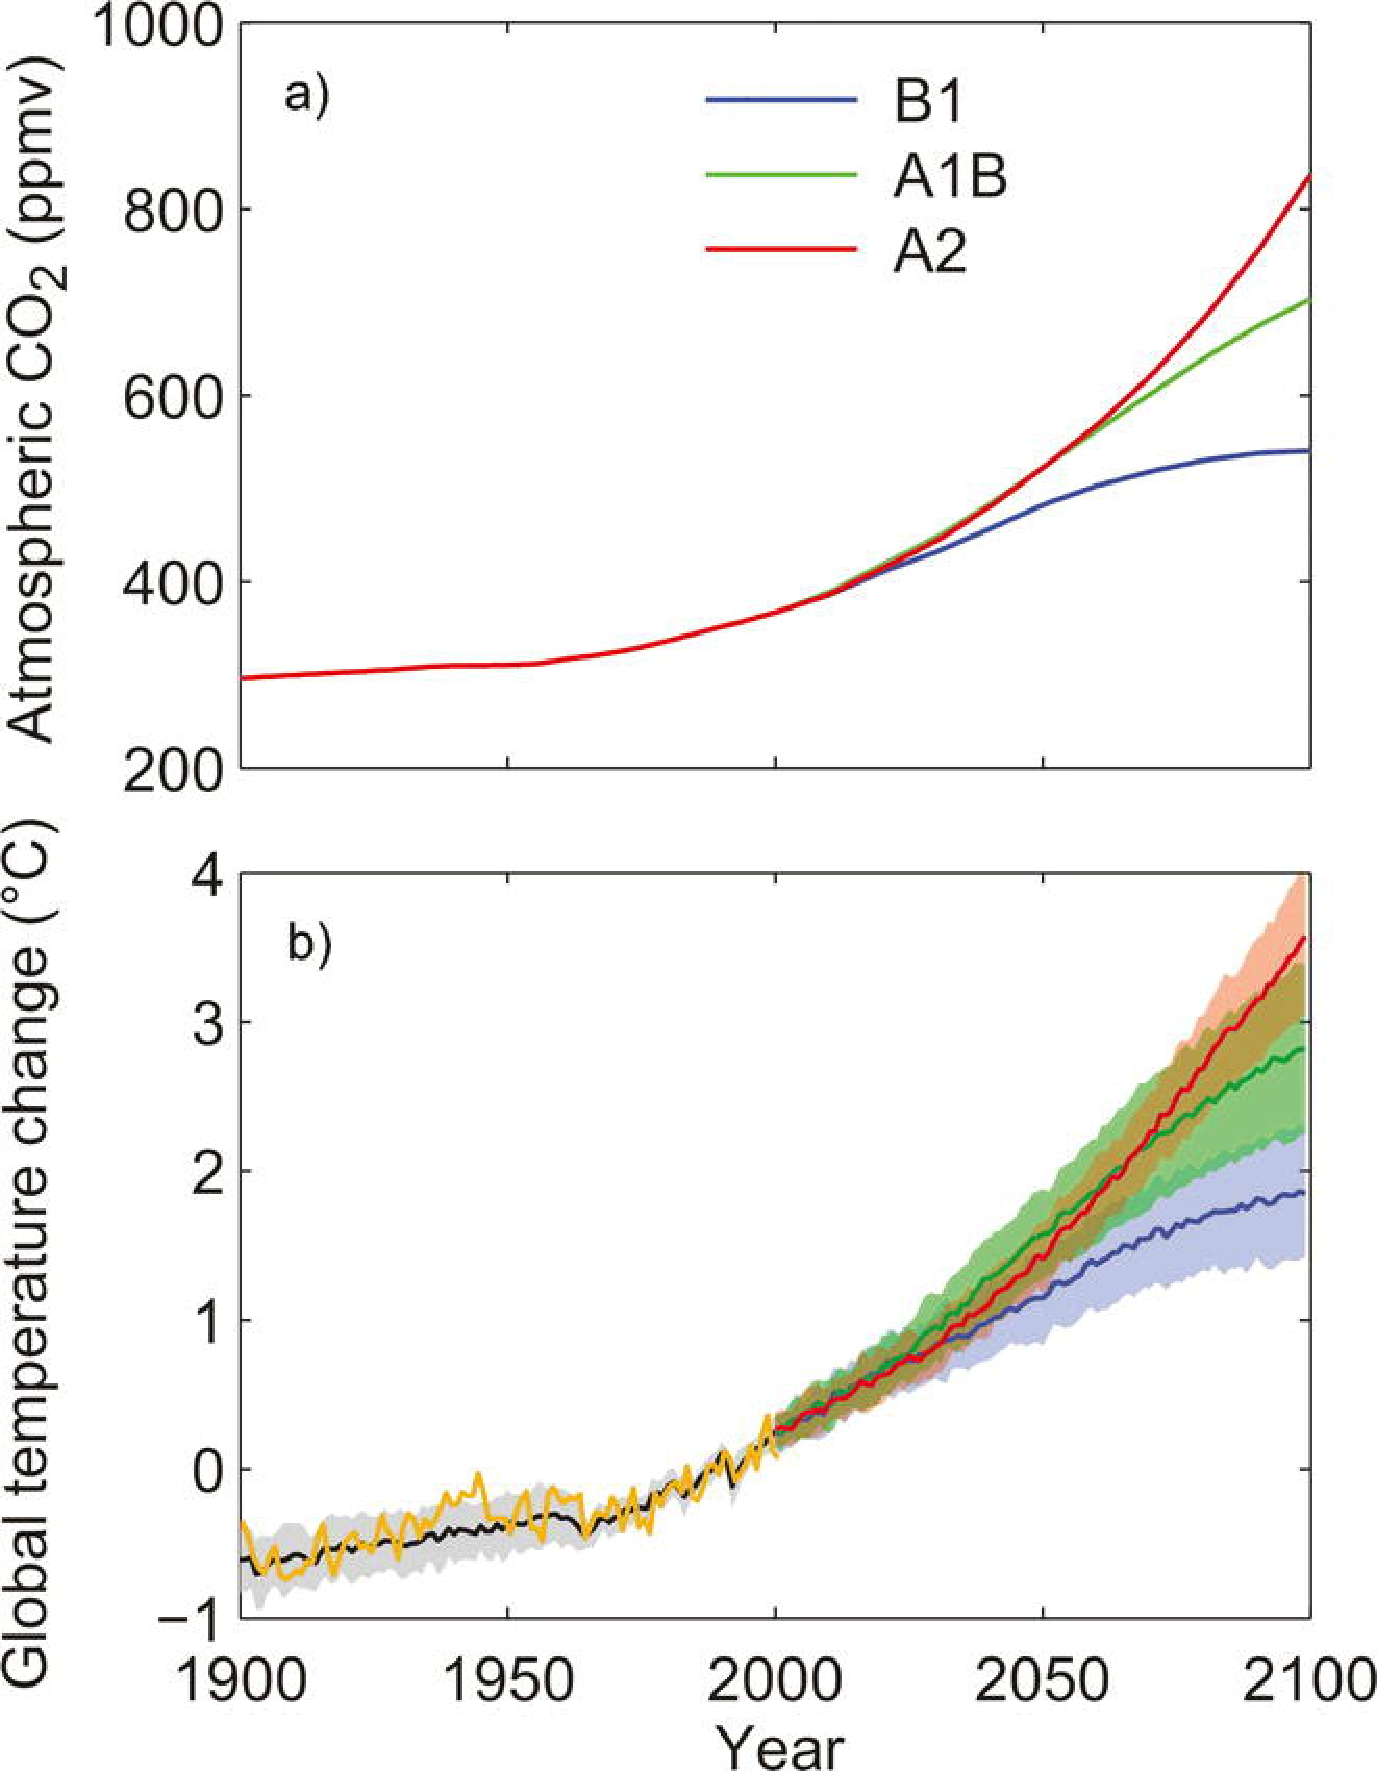
\includegraphics[width=19pc,angle=0]{figure01.pdf}\\
%  \caption{Enter the caption for your figure here.  Repeat as
%  necessary for each of your figures. Figure from \protect\cite{Knutti2008}.}\label{f1}
%\end{figure}

% NOTE: what to include in the paper, key questions.
% The paper should provide insight about what might happen if a large volcano erupted
% (order of magnitude or more than Mt.\ Pinatubo). How does the atmosphere react, for
% example in the aerosol dynamics? (QBO, SO2/AOD/RF relationship.) It should also be
% about how volcanic simulations compare in magnitude and if there is time for more
% simulations, how model complexity (dynamic ocean against slab ocean) affect things.
% - How far does the linear relation between AOD and RF go? What phases does the
%   aerosols go though? (Perhaps the most promising avenue.)
% - How much does it matter how high in the atmosphere the initial SO2 is injected?
%   (Already is some literature on this, suggesting it is not much. Also some on
%   latitude dependence, which has a bigger influence.)
% - How does the climate response change based on the state of the climate: what if we
%   run a CO2 doubling or quadrupling simulation until close to equilibrium, and let the
%   volcanoes erupt then? (Lack the doubling scenario, and setting it up has resulted in
%   strange output that must be resolved. Could take a while.)

\section{Introduction}

% NOTE: Suggested layout for the introduction
% - The objectives of the work.
% - The justification for these objectives: Why is the work important?
% - Background: Who else has done what? How? What have we done previously?
% - Guidance to the reader: What should the reader watch for in the paper? What are the
%   interesting high points? What strategy did we use?
% - Summary/conclusion: What should the reader expect as conclusion? In advanced
%   versions of the outline, you should also include all the sections that will go in
%   the Experimental section (at the level of paragraph subheadings) and indicate what
%   information will go.

% Toohey et al 2011 have a nice end of introduction.

\Gls{rf} and \gls{aod} are crucial metrics representing the energy imbalance at
\gls{toa} and the stratospheric opacity due to aerosol scattering. They are extensively
utilized to quantify the impact of major volcanic eruptions. The assumption of a linear
dependency of \gls{rf} on \gls{aod} is commonly adopted \citep{myhre2013,andersson2015},
and applying such a linear relationship have yielded reasonably accurate estimates in
climate model simulations of volcanic eruptions
\citep{mills2017,hansen2005,gregory2016,marshall2020,pitari2016b}. Despite this, there
is a wide spread in the estimated volcanic forcing efficiencies (\gls{rf} normalised by
\gls{aod}) among the studies, spanning approximately \(\sim
\SI{15}{\watt\metre^{-2}\ce{AOD}^{-1}}\) \citep{pitari2016b} to \(\sim
\SI{25}{\watt\metre^{-2}\ce{AOD}^{-1}}\) \citep{myhre2013}, predominantly based on
\gls{aod} values up to at most \(\sim 0.7\).

Although \ce{H2O}, \ce{N2} and \ce{CO2} are the most abundant gases emitted by volcanoes
\citep{robock2000}, sulphur species such as \ce{SO2} hold greater influence due to the
comparatively high concentrations of the former gases in the atmosphere. The
transformation of \ce{SO2} molecules through reactions with \ce{OH} and \ce{H2O} leads
to the formation of sulphate acis (\ce{H2SO4}) \citep{robock2000}, which scatter
sunlight, elevating planetary albedo and consequently the \gls{rf}. As the conversion
from \ce{SO2} to \ce{H2SO4} occurs over weeks \citep{robock2000}, the peak \gls{rf} from
the eruption experiences a slight delay from the eruption's. The duration of time the
\ce{H2SO4} aerosols stay in the stratosphere depends on various factors, including
latitude \citep{marshall2019, toohey2019}, volcanic plume height \citep{marshall2019},
aerosol size \citep{marshall2019}, \gls{qbo} phase \citep{pitari2016b} and the season of
the year (determining to which hemisphere aerosols are transported)
\citep{toohey2011,toohey2019}. In the case of tropical eruptions, aerosols are typically
transported poleward in the stratosphere and back to mid-latitude troposphere within one
to two years \citep{robock2000}. Upon descending below the tropopause, these aerosols
are readily removed by wet deposition \citep{liu2012}.

Before the current era of significant anthropogenic climate forcing, volcanic eruptions
primarily dictated Earth's climate variability during the Holocene period
\citep{sigl2022}. Despite this substantial impact, few climate model experiments have
included volcanic forcing when simulating climate evolution during the Holocene
\citep{sigl2022}, implying an exaggerated positive forcing
\citep{gregory2016,solomon2011}. This absence of persistent cooling is one of several
factors that has been suggested to contribute to the common disparity between simulated
and observed global warming \citep{andersson2015}. Despite extensive attention on
understanding how volcanic eruptions influence climate, questions regarding aerosol
particle processes---such as their growth and creation rates when \ce{OH} is
scarce---remain unanswered
\citep[e.g.][]{robock2000,zanchettin2019,marshall2020,marshall2022}. These processes
impact aerosol scattering efficiency and potentially the \gls{rf} to \gls{aod}
relationship. \citet{marshall2020} observed higher efficiencies in years \(2\) and \(3\)
post-eruption compared to year 1, attributing this to spatial concentration in the
initial year and subsequent dispersion. This spatial alteration increases the albedo per
global mean \gls{aod}, consequently elevating the \gls{rf} to \gls{aod} ratio
\citep{marshall2020}.

Previous studies on both Mt.\ Pinatubo \citep{mills2017,hansen2005} and volcanoes within
the instrumental era \citep{gregory2016} have been used to estimate the relationship
between the \gls{rf} energy imbalance and change in \gls{aod} caused by volcanic
eruptions. While \citet{myhre2013} employ a \gls{rf} formula scaling \gls{aod} by
\(\SI{-25}{\watt\metre^{-2}\mathrm{AOD}^{-1}}\), recent literature reports estimates
down to \(\SI{-19.0(5)}{\watt\metre^{-2}\mathrm{AOD}^{-1}}\) \citep{gregory2016} and
\(\SI{-18.3(10)}{\watt\metre^{-2}\mathrm{AOD}^{-1}}\) \citep{mills2017}. Synthetic
volcano simulations in \citet{marshall2020} yield a scaling factor of
\(\SI{-20.5(2)}{\watt\metre^{-2}\mathrm{AOD}^{-1}}\) across 82 simulations featuring
varying injection heights and latitudes of volcanic emissions, ranging from \(10\) to
\(\SI{100}{\tera\gram(\ce{SO2})}\).

A similar simulation setup, albeit with notable differences, was conducted by
\citet{niemeier2015}, involving \(14\) levels of injected sulphur spanning between
\(\SI{1}{\tera\gram(\ce{S})\mathrm{yr}^{-1}}\)
(\(\SI{2}{\tera\gram(\ce{SO2})\mathrm{yr}^{-1}}\)) and
\(\SI{100}{\tera\gram(\ce{S})\mathrm{yr}^{-1}}\)
(\(\SI{200}{\tera\gram(\ce{SO2})\mathrm{yr}^{-1}}\)). These geoengineering simulations
maintained continous sulphur injections, running until a steady sulphur level was
achieved. Results indicated an inverse exponential relationship between \gls{rf} and
\iso{} rate, converging to \(\SI{-65}{\watt\metre^{-2}}\)
(eq.~\ref{eq:niemeier_exponential}). Notably, even though the super-volcano simulation
by \citet{jones2005} have a much weaker gradient of \(\sim
\SI{-4}{\watt\metre^{-2}\mathrm{AOD}^{-1}}\) when compared to more recent literature,
the peak \gls{rf} obtained in their simulation was \(\SI{-60}{\watt\metre^{-2}}\), still
below the suggested limit of \(\SI{-65}{\watt\metre^{-2}}\). Moreover,
\citet{timmreck2010} find a peak \gls{rf} anomaly of \(\SI{-18}{\watt\metre^{-2}}\) from
\(\SI{1700}{\tera\gram(\ce{SO2})}\), which corresponds well with the function estimated
by \citet{niemeier2015}.

One avenue that has garnered considerable attention is comparing the magnitude of
forcing from volcanoes or volcano-like forcings compared to increased \ce{CO2} levels.
Several studies explore the connection between volcanic forcing and the climate
sensitivity to a doubling of \ce{CO2}
\citep{boer2007,marvel2016,merlis2014,ollila2016,richardson2019,salvi2022,wigley2005}.
This comparison aims to mitigate the large uncertainty in estimates of the sensitivity
of the real climate system. Inferring climate sensitivity from volcanic events has been
attempted as a means of constraining the sensitivity \citep{boer2007}, assuming that
volcanic and \ce{CO2} forcings produce similar feedbacks \citep{pauling2023}. Earlier
studies suggest the potential for constraining \gls{ecs} using volcanoes
\citep{bender2010}, provided that \gls{ecs} is constrained by \gls{erf} rather than
\gls{irf}, as \gls{erf} accounts for rapid atmospheric adjustments in contrast to
\gls{irf} \citep{richardson2019}. However, other studies refute this by indicating
different sensitivities between volcanic forcing and \ce{CO2} doubling
\citep{douglass2006} or asserting that constraining the \gls{ecs} by \gls{erf} lacks
accuracy due to the precision of climate simulations \citep{boer2007,salvi2022}.
Although \gls{erf} offers a more suitable indicator of forcing than \gls{irf}
\citep{marvel2016,richardson2019}, more recent studies conclude that \gls{ecs} cannot be
constrained from volcanic events \citep{pauling2023}.

Several studies have demonstrated a linear relationship of approximately
\(-\SI{20}{\watt\metre^{-2}\mathrm{AOD}^{-1}}\) between \gls{rf} and \gls{aod}, although
substantial variability exists in the slope among studies
\citep{mills2017,hansen2005,gregory2016,marshall2020,pitari2016b}. Moreover, a
time-after-eruption dependence on the \gls{rf} to \gls{aod} ratio is found in
\citet{marshall2020}, whereas \citet{niemeier2015} revealed a non-linear relationship
between \gls{rf} and \iso{}. Thus, a consensus on the relationship between \iso{},
\gls{aod} and \gls{rf} has yet to be established.

To address these issues we conducted ensemble simulations of volcanic eruptions in
\gls{cesm2}, spanning \iso{} levels of three orders of magnitude:
\(\SI{26}{\tera\gram(\ce{SO2})}\), \(\SI{400}{\tera\gram(\ce{SO2})}\) and
\(\SI{1629}{\tera\gram(\ce{SO2})}\). Details regarding the experimental setup are
provided in section~\ref{sec:method}. Our finding reveal clear non-linear \gls{rf} to
\gls{aod} dependencies for large to super-volcano scale eruptions. Additionally, we
observe a time-dependent variation in the \gls{rf} to \gls{aod} ratio, detailed in
section~\ref{sec:results} and discussed in section~\ref{sec:discussion}. Furthermore,
our data, along with insights from previous studies, suggest that the \gls{rf} to \iso{}
dependency identified by \citet{niemeier2015} acts as a lower boundary. Our conclusions
are presented in section~\ref{sec:conclusions}.

\section{Method}\label{sec:method}

\subsection{Model}

% TODO: decide if this table is useful at all (probably not)
% \begin{table*}
%   \centering
%
%   \caption{\glsentrylong{cesm2} model components}\label{tab:cesm-components}%
%   \begin{center}
%     \begin{tabular}[c]{ll}
%       \multicolumn{1}{c}{Component name} &
%       \multicolumn{1}{c}{Reference}                                              \\
%       \glsentrylong{cesm2}               & \citet{danabasoglu2020}               \\
%       \glsentrylong{waccm}               & \citet{gettleman2019}                 \\
%       \glsentrylong{pop}                 & \citet{smith2010, danabasoglu2020}    \\
%       \glsentrylong{mosart}              & \citet{li2013, danabasoglu2020}       \\
%       \glsentrylong{clm}                 & \citet{lawrence2019, danabasoglu2020} \\
%       \glsentrylong{ww3}                 & \citet{danabasoglu2020}               \\
%       \glsentrylong{cice}                & \citet{danabasoglu2020}               \\
%       \glsentrylong{cism}                & \citet{danabasoglu2020}               \\
%       \glsentrylong{cime}                & \citet{danabasoglu2020}               \\
%     \end{tabular}
%   \end{center}
% \end{table*}

We utilized the \gls{cesm2} \citep{danabasoglu2020} in conjunction with the \gls{waccm}
\citep{gettleman2019} and the fully dynamical ocean component \gls{pop}
\citep{smith2010, danabasoglu2020}. The atmosphere model was run at nominal
\(\SI{2}{\degree}\) resolution with \(70\) vertical levels in the \gls{ma}
configuration.

The \gls{waccm} version employed in the \gls{ma} configuration uses the \gls{mam3}
\citep{gettleman2019}, a simplified and computationally efficient default setting within
the \gls{cam5} \citep{liu2016}, as described in \citet{liu2012}. The \gls{mam3} was
developed from MAM7, consisting of the seven modes Aitken, accumulation, primary carbon,
fine dust and fine sea salt, coarse dust and coarse sea salt. Instantaneous internal
mixing of primary carbonaceous aerosols with secondary aerosols and instantaneous ageing
of primary carbonaceous particles is assumed by emitting primary carbon in the
accumulation mode \citep{liu2016}. Fine sea salt is assimilated into the accumulation
mode, and as dust absorbs water efficiently it is expected to be removed by wet
deposition similarly to sea salt, allowing fine dust to be merged into the accumulation
mode as well. Likewise, coarse dust is merged with coarse sea salt into a coarse mode,
and as both absorb water efficiently, the coarse mode will quickly retain its background
state below the tropopause \citep{liu2012}. Consequenctly, \gls{mam3} features three
modes: Aitken, accumulation and coarse \citep{liu2016}.

\subsection{Simulations}

Appendix A provides a detailed description of the simulation setup and utilized output
variables. Table~\ref{tab:simulation-overview} summarizes the simulations, encompassing
three \ce{SO2} injection magnitudes across four seasons: February 15th, May 15th, August
15th, and November 15th. The magnitudes vary over three orders of magnitude:
\(\SI{26}{\tera\gram(\ce{SO2})}\), \(\SI{400}{\tera\gram(\ce{SO2})}\), and
\(\SI{1629}{\tera\gram(\ce{SO2})}\).

The smallest eruption case (\gls{c2wm}) aligns with the magnitude of events like Mt.\
Pinatubo \citep[\(\sim10\)--\(\SI{20}{\tera\gram(\ce{SO2})}\);~e.g.][]{timmreck2018} and
Mt.\ Tambora \citep[\(\sim\SI{56.2}{\tera\gram(\ce{SO2})}\);~e.g.][]{zanchettin2016}.
The intermediate case (\gls{c2wmp}) resembles the 1257 Samalas eruption
\citep[\(\sim{118.8}\)--\(\SI{173.1}{\tera\gram(\ce{SO2})}\);~e.g.][]{toohey2017,ottobliesner2016},
while the largest eruption case (\gls{c2ws}) is similar to the \gls{ytt} eruption
\citep[\(100\)--\(\SI{10000}{\tera\gram(\ce{SO2})}\);~e.g.][]{jones2005}. All eruptions
were situated at the equator (\(\SI{0}{\degree N}\), \(\SI{1}{\degree E}\)) with
\ce{SO2} injected between \(\SI{18}{\kilo\meter}\) and \(\SI{20}{\kilo\meter}\).
Collectively, the three eruption cases \gls{c2wm}, \gls{c2wmp} and \gls{c2ws} are
referred to as \gls{c2w}. Two additional high-latitude eruptions (\gls{c2wsn}) of the
same \iso{} magnitude as \gls{c2ws} were simulated at \(\SI{56}{\degree N}\),
\(\SI{287.7}{\degree E}\) with a six-month separation (February 15th and August 15th).

Employing eruptions in the large to super-volcano size enhances the signal-to-noise
ratio without necessitating an extensive and computationally expensive ensemble.
However, the forcing values obtained from the climate model simulations may not be
realistic or more specifically an appropriate representation of smaller eruptions
typical of the historical period \citep{gregory2016}.
% TODO: Mention this in relation to the different ratios for eruption size? In relation
% to J05 and my calculations of climate resistance.

\begin{table*}
  \centering

  \caption{Simulations done with the \gls{cesm2}. \gls{c2wsn} and \gls{c2ws} are the same
    in eruption magnitude, but while \gls{c2ws} is located at the equator, \gls{c2wsn} is
    located at high latitude. \gls{c2wmp} and \gls{c2wm} are located at the equator, but
    with different magnitudes to \gls{c2ws}}\label{tab:simulation-overview}%
  \begin{center}
    \begin{tabular}[c]{cccc}
      Name           & \(\si{\tera\gram(\ce{SO2})}\)         & Lat, lon, alt [\si{\degree\mathrm{N}}, \si{\degree\mathrm{E}}, \si{\kilo\metre}] &
      Eruption months                                                                                                                             \\
      \gls{c2wsn}    & \(1629\)                              &
      \(56\), \(287.7\),
      \(18\)--\(20\) & Feb,\hphantom{May,}Aug\hphantom{,Nov}                                                                                      \\
      \gls{c2ws}     & \(1629\)                              &
      \(\hphantom{1}0\), \(\hphantom{28}1\hphantom{.7}\), \(18\)--\(20\)
                     & Feb,May,Aug,Nov                                                                                                            \\
      \gls{c2wmp}    & \(\hphantom{1}400\)                   &
      \(\hphantom{1}0\),
      \(\hphantom{28}1\hphantom{.7}\),
      \(18\)--\(20\) & Feb,May,Aug,Nov                                                                                                            \\
      \gls{c2wm}     & \(\hphantom{14}26\)                   &
      \(\hphantom{1}0\),
      \(\hphantom{28}1\hphantom{.7}\), \(18\)--\(20\)
                     & Feb,May,Aug,Nov                                                                                                            \\
    \end{tabular}
  \end{center}
\end{table*}

\section{Results}\label{sec:results}

% NOTE: the results should be laid out in a logical way, with the most
% interesting/important stuff first, then tangents that dig deeper at specific things
% later.
% 1. RF to AOD time-after-eruption dependence should be top priority (8 figs atm.)
% 2. Then probably temperature scaling since we discuss the shape of both AOD and RF
%    time series before that (MOTIVATION: can we expect a specific temperature time
%    series shape based on the shape of either of or both of the RF and AOD time
%    series?)
% 3. If there is something interesting to say about the rest of the figures (all the
%    comparing of parameters), then this should come here.

\subsection{Analysis of the time series}

Fig.~\ref{fig:compare-waveform-temp} illustrates time series of the global mean
\gls{aod}, \gls{rf}, and surface air temperature. The black lines represent the medians
across the four-member ensembles, while shading indicates the 5th to 95th percentiles.
Three distinct forcing magnitudes (\gls{c2wm}, \gls{c2wmp}, and \gls{c2ws}), outlined in
table~\ref{tab:simulation-overview}, have been used. The time series in
fig.~\ref{fig:compare-waveform-temp} are normalised by setting the peak value to unity,
defined based on the peak of a fit utilising a Savitzky-Golay filter of 3rd order and a
one-year window length.

A notable feature across all three subfigures of fig.~\ref{fig:compare-waveform-temp} is
the earlier peak occurrence of the \gls{c2wm} case compared to the larger eruption
cases. Cases \gls{c2wmp} and \gls{c2ws} peak at similar times, but the \gls{c2wmp} case
exhibit a faster rise in the \gls{aod} time series
(fig.~\ref{fig:compare-waveform-temp}a). Additionally in
fig.~\ref{fig:compare-waveform-temp}a we find that the stronger eruption cases display a
sharper peak, or similarly a slower rise and faster decay. The rise across the eruption
cases in fig.~\ref{fig:compare-waveform-temp}b is similar, but where the \gls{c2wm} case
reach the peak just prior to the other two cases. Although the rise in the eruption
cases in fig.~\ref{fig:compare-waveform-temp}b is similar, the \gls{c2wm} case reaches
its peak just before the other two cases. During the decay phase, all cases appear to
decay at a similar rate, maintaining the offset caused by the earlier peak arrival of
\gls{c2wm}. Cases \gls{c2wmp} and \gls{c2ws} exhibit indistinguishable \gls{rf} time
series. Similarly, in fig.~\ref{fig:compare-waveform-temp}, when observing the
temperature evolution, cases \gls{c2wmp} and \gls{c2ws} are indistinguishable. The
\gls{c2wm} case spends less time around the peak but decays much faster compared to the
\gls{c2wmp} and \gls{c2ws} cases.

Across all cases in each of the parameters shown in
fig.~\ref{fig:compare-waveform-temp}, no non-linear effects appear to have an impact,
even in the \gls{c2ws} super-volcano case. Comparing the two strongest eruption cases
(\gls{c2wmp} and \gls{c2ws}), where noise play a much smaller role, the \gls{rf} and
temperature time series are indistinguishable from each other. Therefore, similar
dynamics are expected to be at play in all cases.

\begin{figure}
  \centering
  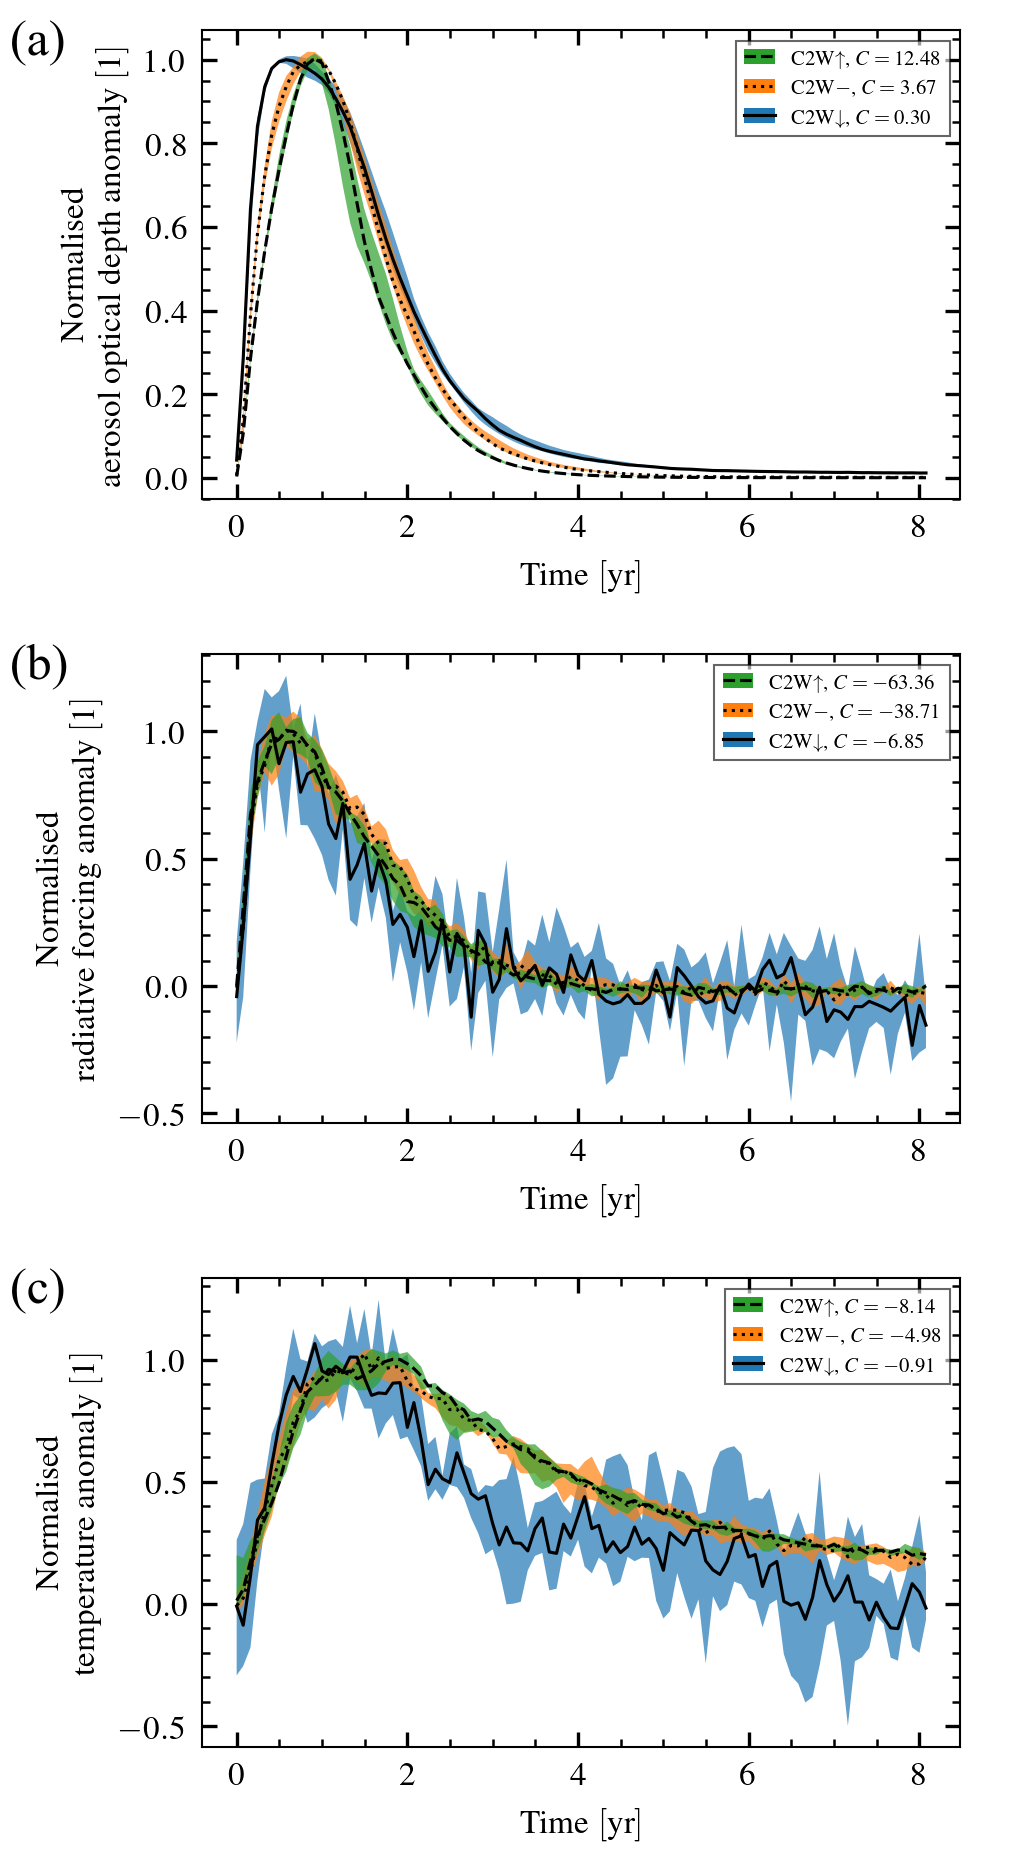
\includegraphics{figures/figure1.png}

  \caption{\gls{aod} (a), \gls{rf} (b) and temperature response (c) time series to the
    three tropical volcanic eruption cases, \gls{c2wm}, \gls{c2wmp} and \gls{c2ws}. The time
    series have been normalised to have peak values at unity, where \(C\) is the
    normalisation constant. Black lines indicate the median across the four-member
    ensembles, while shading marks the 5th and 95th
    percentiles.}\label{fig:compare-waveform-temp}%
\end{figure}

Next, we investigate whether the shape of the temperature time series can be inferred
from the shape of either of the forcing time series (\gls{aod} or \gls{rf}). When
plotting the \gls{rf} time series, we find that their shapes are consistent over
different eruption strengths (fig.~\ref{fig:compare-waveform-temp}b), suggesting a
strong dependence of temperature on \gls{rf}. The same can largely be said about the
\gls{aod} time series as well, but they do show a slight change in shape from smaller to
larger eruptions (fig.~\ref{fig:compare-waveform-temp}a). Specifically, the \gls{aod}
time series from smaller eruptions display a fast rise and a flat peak before decaying
back to their equilibrium state. From the larger eruptions, we find a slower rise time
but a sharper peak, resulting in a decay to equilibrium happening at a similar time
after the eruption and at a similar rate.

\subsection{\gls{rf} dependency on \gls{aod}}

We next focus on how the \gls{aod} and \gls{rf} time series develop relative to each
other. Similar comparisons were conducted in \citet[][their Fig.\ 4]{gregory2016} and
\citet[][their Fig.\ 1]{marshall2020}, with \gls{rf} plotted against \gls{aod}.
Fig.~\ref{fig:aod_vs_toa_ses_avg} displays annual mean values from the four simulation
cases in table~\ref{tab:simulation-overview}; the small eruption case (\gls{c2wm}) as
blue downward pointing triangles, the intermediate eruption case (\gls{c2wmp}) as orange
thick diamonds, the large tropical eruption case (\gls{c2ws}) as green upward pointing
triangles, and the large northern hemisphere eruption case (\gls{c2wsn}) as brown upward
pointing three-branched twigs. Also shown are the data from \citet[][Fig.\ 4, black
  crosses from HadCM3 sstPiHistVol]{gregory2016} as grey crosses labelled \gls{g16}.
Additionally, the estimated peak values from the Mt.\ Pinatubo and Mt.\ Tambora
eruptions are plotted as a purple star and a yellow plus, while the peak from the
\gls{j05} simulation is shown as a pink square. Finally, red circles represent the peak
values obtained from the \gls{c2w} tropical eruption cases. The gradient lines are the
same as shown by \citet{gregory2016}. The full data range is shown in
fig.~\ref{fig:aod_vs_toa_ses_avg}a while fig.~\ref{fig:aod_vs_toa_ses_avg}b highlights a
narrow range, focusing on the \gls{c2wm} case.

The annual mean data from the Pinatubo-like \gls{c2wm} case in
fig.~\ref{fig:aod_vs_toa_ses_avg}b have \gls{rf} values as a function of \gls{aod} that
follow almost the same constant gradient as the \gls{g16} data. However, in
fig.~\ref{fig:aod_vs_toa_ses_avg}a we observe that the stronger eruptions lead to
dissimilar responses in \gls{aod} and \gls{rf}, where the slope of the \gls{c2wmp} case
seems to follow close to a \(-10\) gradient and the \gls{c2ws} case is closer to a
\(-5\) gradient. The peak values (red circles) suggest a non-linear functional shape
dependence, while within each eruption strength (same colour) the annual mean values
fall relatively close to a straight line.

\begin{figure}
  \centering
  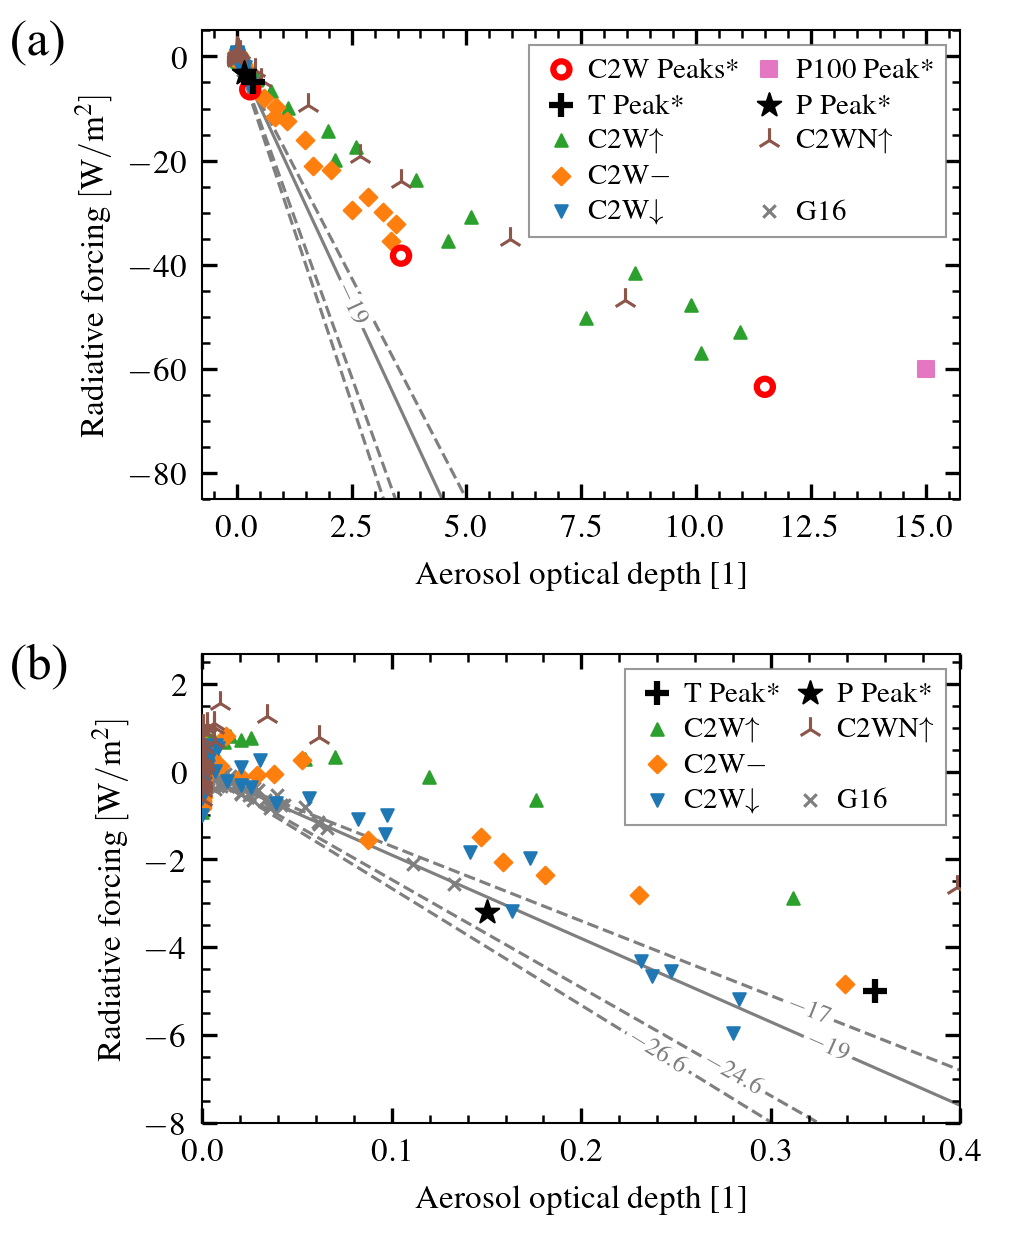
\includegraphics{figures/figure2.png}

  \caption{\gls{rf} as a function of \gls{aod}, yearly means. Data from the four
    simulations listed in table~\ref{tab:simulation-overview} (\gls{c2wm}, \gls{c2wmp},
    \gls{c2ws} and \gls{c2wsn}) are shown along with the data from the HadCM3 sstPiHistVol
    simulation by \citet{gregory2016} (grey crosses). Also shown are the estimated peak
    values of the Mt.\ Pinatubo (purple star) and Mt.\ Tambora (yellow plus) eruptions. In
    (a) the simulated super-volcano of \citet{jones2005} (pink square) is shown as well as
    the peak values from the simulations \gls{c2wm}, \gls{c2wmp} and \gls{c2ws} as red
    circles. All peak values (as opposed to annual means) have an asterisk (\(\ast{}\)) in
    their label. The grey gradient lines are the same regression fits as in \citet[][Fig.\
      4]{gregory2016}, where the solid line is the fit to the Gregory et al.\ data (grey
    crosses). (b): Zooming in on the smallest values.}\label{fig:aod_vs_toa_ses_avg}%
\end{figure}

To observe how the responses in \gls{aod} and \gls{rf} develop relative to each other
over time, we plot in fig.~\ref{fig:aod_vs_toa_avg_loop_ratios} seasonal means of the
\gls{rf} to \gls{aod} ratio, where the start of the time series is taken as that of the
eruption day. The plot shows all the eruption cases given in
table~\ref{tab:simulation-overview}, as well as the tropical eruptions from the
\citet{marshall2020dataset} dataset, labelled \gls{m20}. In
fig.~\ref{fig:aod_vs_toa_avg_loop_ratios}a, straight lines are linear regression fits to
the seasonal means across all four ensembles, summarised in
table~\ref{tab:slope-gradients}. Shaded regions are the standard deviation around the
seasonal means. A similar shading is plotted in
fig.~\ref{fig:aod_vs_toa_avg_loop_ratios}b, but where the regression fits have been
omitted to avoid further cluttering the plot. The years where the signal-to-noise ratio
is the lowest are years \(1\) and \(2\), as well as year \(0\) (the noise is mostly due
to the \gls{rf} time series, shown in fig.~\ref{fig:compare-waveform-temp}b). For this
reason, the ratio of \gls{rf} to \gls{aod} is calculated for the second season of the
first year until the end of the third year.

Although the ratio changes between the eruption magnitudes, we find that the gradient at
which the ratio is changing is similar across large eruption magnitudes, summarised in
table~\ref{tab:slope-gradients}. A slope of around \(4\)--\(5\) during the first period
is a good fit for both the \gls{c2wmp} case and the \gls{c2ws} case
(table~\ref{tab:slope-gradients}, row ``fig.~\ref{fig:aod_vs_toa_avg_loop_ratios}a''),
and even though the spread in the \gls{c2wm} case is large in the \(y\)-direction, they
tend to follow a similarly inclined, albeit steeper, slope. Normalising the time series
before computing the ratio, shown in fig.~\ref{fig:aod_vs_toa_avg_loop_ratios}b, yields
a similarly inclined slope across all forcing magnitude ensembles except the \gls{c2wsn}
case at high latitude. In the 2nd period, from the second season of the second year, the
ratios stay close to constant for the reminder of the decaying phase of the time series.
Again, this is necessarily the case also in the normalised version in
fig.~\ref{fig:aod_vs_toa_avg_loop_ratios}b, but here the effect of a smaller
signal-to-noise ratio into the third year becomes apparent.

\begin{table}
  \centering

  \caption{Gradient and standard deviation for the regression lines to the data found in
    fig.~\ref{fig:aod_vs_toa_avg_loop_ratios}. The regression fit in the top half of the
    table indicate the regression fits to fig.~\ref{fig:aod_vs_toa_avg_loop_ratios}a, while
    the bottom half is the regression fits to fig.~\ref{fig:aod_vs_toa_avg_loop_ratios}b.
    The columns ``1st period'' and ``2nd period'' refer to the period from year \(0\) to
    year \(1\)) and the period from year \(1\) to year \(3\)}\label{tab:slope-gradients}%
  \begin{tabular}{cccc}
    Figure               & Simulation  & 1st period      & 2nd period       \\
    \rowcolor{LightGray} & \gls{c2wsn} & \(0.34\pm1.20\) & \(0.68\pm1.34\)  \\
    \rowcolor{LightGray} & \gls{c2ws}  & \(4.00\pm0.52\) & \(-3.00\pm0.55\) \\
    \rowcolor{LightGray} & \gls{c2wmp} & \(4.84\pm0.83\) & \(-2.76\pm0.46\) \\
    \rowcolor{LightGray} & \gls{c2wm}  & \(9.22\pm2.67\) & \(-0.55\pm2.51\) \\
    \rowcolor{LightGray} & \gls{m20}   & \(6.34\pm1.77\) & \(-0.36\pm1.33\) \\
    \multirow{5}{*}{4b}  & \gls{c2wsn} & \(0.06\pm0.21\) & \(0.12\pm0.24\)  \\
    \multirow{-9}{*}{4a} & \gls{c2ws}  & \(0.78\pm0.10\) & \(-0.59\pm0.11\) \\
                         & \gls{c2wmp} & \(0.48\pm0.08\) & \(-0.28\pm0.05\) \\
                         & \gls{c2wm}  & \(0.43\pm0.13\) & \(-0.03\pm0.12\) \\
                         & \gls{m20}   & \(0.33\pm0.07\) & \(-0.02\pm0.08\) \\
  \end{tabular}
\end{table}

\citet[][their Fig.\ 1c,d]{marshall2020} present results that demonstrate a
time-dependent relationship in the conversion between \gls{aod} and \gls{rf}. Contrary
to the results from the \gls{cesm2} simulations, \gls{rf} displays larger magnitudes
compared to \gls{aod} at later stages in the eruption evolution (higher efficiency), not
smaller. This phenomenon is explained by \citet{marshall2020} as the aerosols initially
being spatially confined to the hemisphere where the eruption occurred. Subsequently,
during the second and third years, they spread globally, resulting in a higher global
mean albedo per \gls{aod} and consequently larger \gls{rf} per \gls{aod}. When a similar
analysis to that in fig.~\ref{fig:aod_vs_toa_avg_loop_ratios}a is applied to the
\gls{m20} data (utilised by \citet{marshall2020}), considering eruptions between \(-10\)
and \(\SI{10}{\degree\mathrm{N}}\), the ratio increases similarly to the \gls{c2wmp}
case rather than decreasing. The slopes observed are approximately
\(\sim\SI{6.34}{\watt\metre^{-2}\mathrm{AOD}^{-1}}\) and
\(\sim\SI{-0.36}{\watt\metre^{-2}\mathrm{AOD}^{-1}}\), akin to the \gls{c2wm} case.
Additionally, we note that the slope obtained from our high-latitude case exhibits a
significantly weaker slope than the tropical cases, aligning with the \gls{m20} data.
Considering the \gls{m20} data and the results depicted in
fig.~\ref{fig:aod_vs_toa_avg_loop_ratios}, it appears that various and competing effects
determine the values of \gls{aod} and \gls{rf}, with latitude playing a pivotal role.

The change in ratio, where the smallest ratio corresponds to larger eruptions and the
largest ratio corresponds to smaller eruptions, aligns with the shift observed in peak
values as illustrated in fig.~\ref{fig:aod_vs_toa_ses_avg}a. Here, the red circles
indicate that the peak values saturate in \gls{rf}. The peak magnitudes of \gls{rf}
increase at a slower rate compared to the \gls{aod} peak magnitudes, which rise almost
linearly with \iso{} (also visible in fig.~\ref{fig:parameter_scan}a). This trend might
be due to larger aerosols having time to develop as the amount of \iso{} increases
\citep{niemeier2015,marshall2019}. Consequently, this leads to smaller eruptions'
forcing being more efficient than that of large eruptions, as larger aerosols scatter
radiation less efficiently, resulting in a smaller \gls{rf} to \gls{aod} ratio.

\begin{figure}
  \centering
  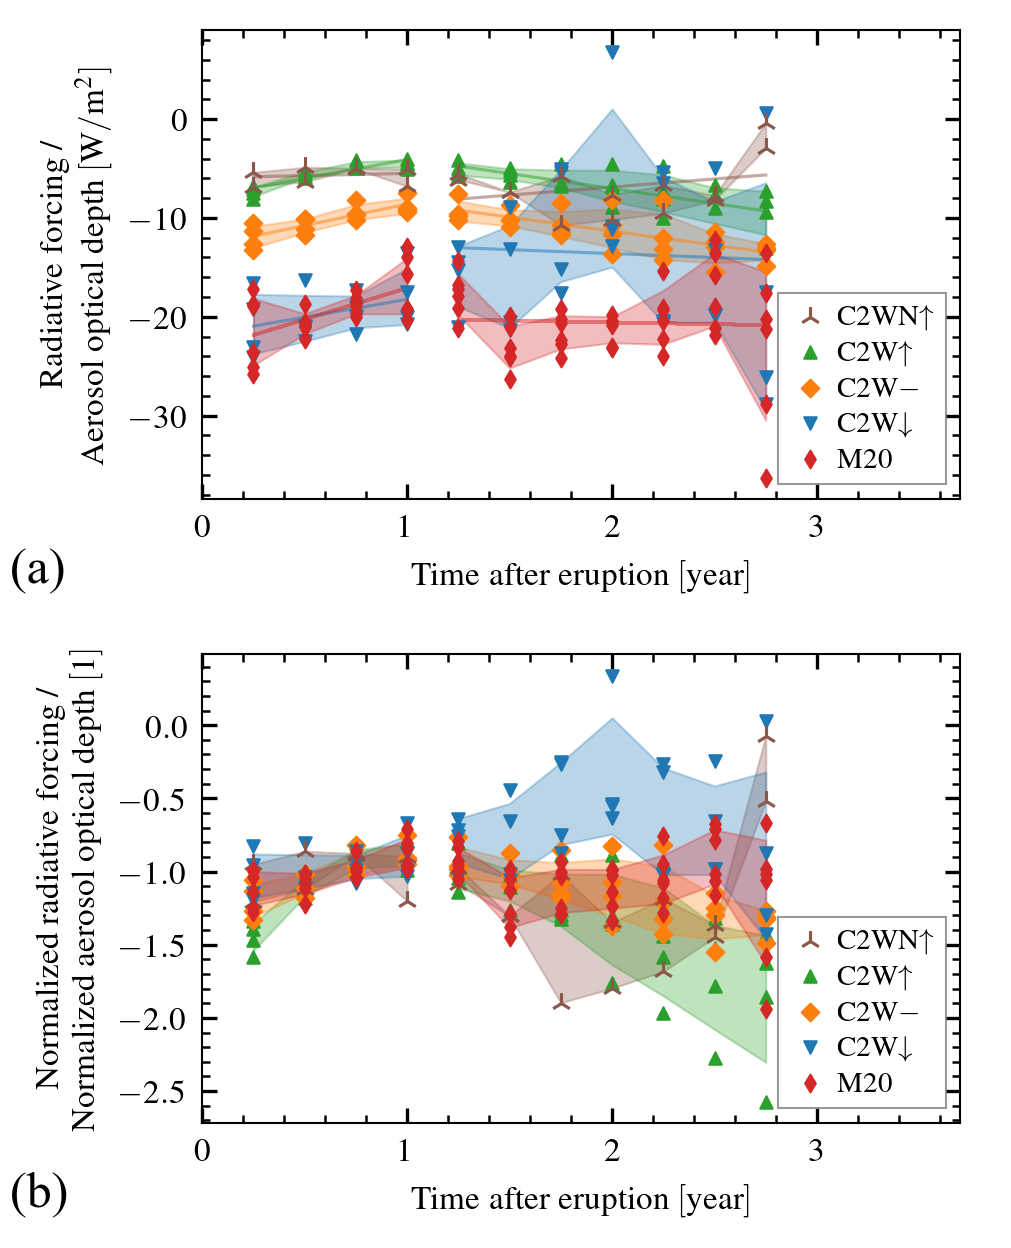
\includegraphics{figures/figure3.png}

  \caption{(a): Ratio of \gls{rf} to \gls{aod}, with time-after-eruption on the horizontal
    axis. Slopes are linear regression fits and are described in
    table~\ref{tab:slope-gradients}, while shaded regions are the standard deviation across
    the ensembles for each season. (b): Same as in (a), but where the underlying \gls{aod}
    and \gls{rf} time series have been scaled to have peak values at unity. Shown are data
    from table~\ref{tab:simulation-overview} along with tropical eruptions from
    \gls{m20}.}\label{fig:aod_vs_toa_avg_loop_ratios}%
\end{figure}

\subsection{Parameter scan}

In fig.~\ref{fig:parameter_scan}, we compare all relevant parameters against each other.
The primary input parameter in the \gls{cesm2} is \iso{}. For out tropical cases
(\gls{c2w}), shown in fig.~\ref{fig:parameter_scan}a, we observe an almost linear
relationship between \gls{aod} peak values and \iso{}. The latitude also play a role for
the extent of the \gls{aod} perturbation, evident from the \gls{c2wsn} data point. This
latitude dependence aligns with findings by \citet{marshall2019}, indicating that
\(\SI{72}{\percent}\) of the \gls{aod} variance can be attributed to \iso{}, while
latitude accounts for only \(\SI{16}{\percent}\) of the variance. Peak values from their
data (82 simulations) plotted as green thin diamonds displays a similar pattern, with
\gls{aod} exhibiting close to linear dependence on \iso{}, but where latitude introduce
a spread in \gls{aod}. Peak values from Mt.\ Pinatubo (P) and Mt.\ Tambora (T) are shown
for reference, along with peak values from \gls{j05} and \gls{t10}.

The almost linear relationship between \gls{aod} and \iso{} for the \gls{c2w} data
suggest a comparable trend for \gls{rf} versus \iso{} as seen in \gls{rf} versus
\gls{aod}. In fig.~\ref{fig:parameter_scan}b, \gls{rf} plotted against \iso{} (with the
absolute value of \gls{rf} on the \(y\)-axis) indicates a substantial damping effect on
\gls{rf} as \iso{} increases, akin to the behaviour seen in the \gls{ob16} data. The
analysis details of the \gls{ob16} data can be found in Appendix B. Despite the model
complexity difference, \citet{ottobliesner2016}'s simulations using \gls{cesm1} with a
low-top atmosphere (\gls{cam5}) produce \glspl{rf} comparable to out findings.

\begin{figure*}
  \centering
  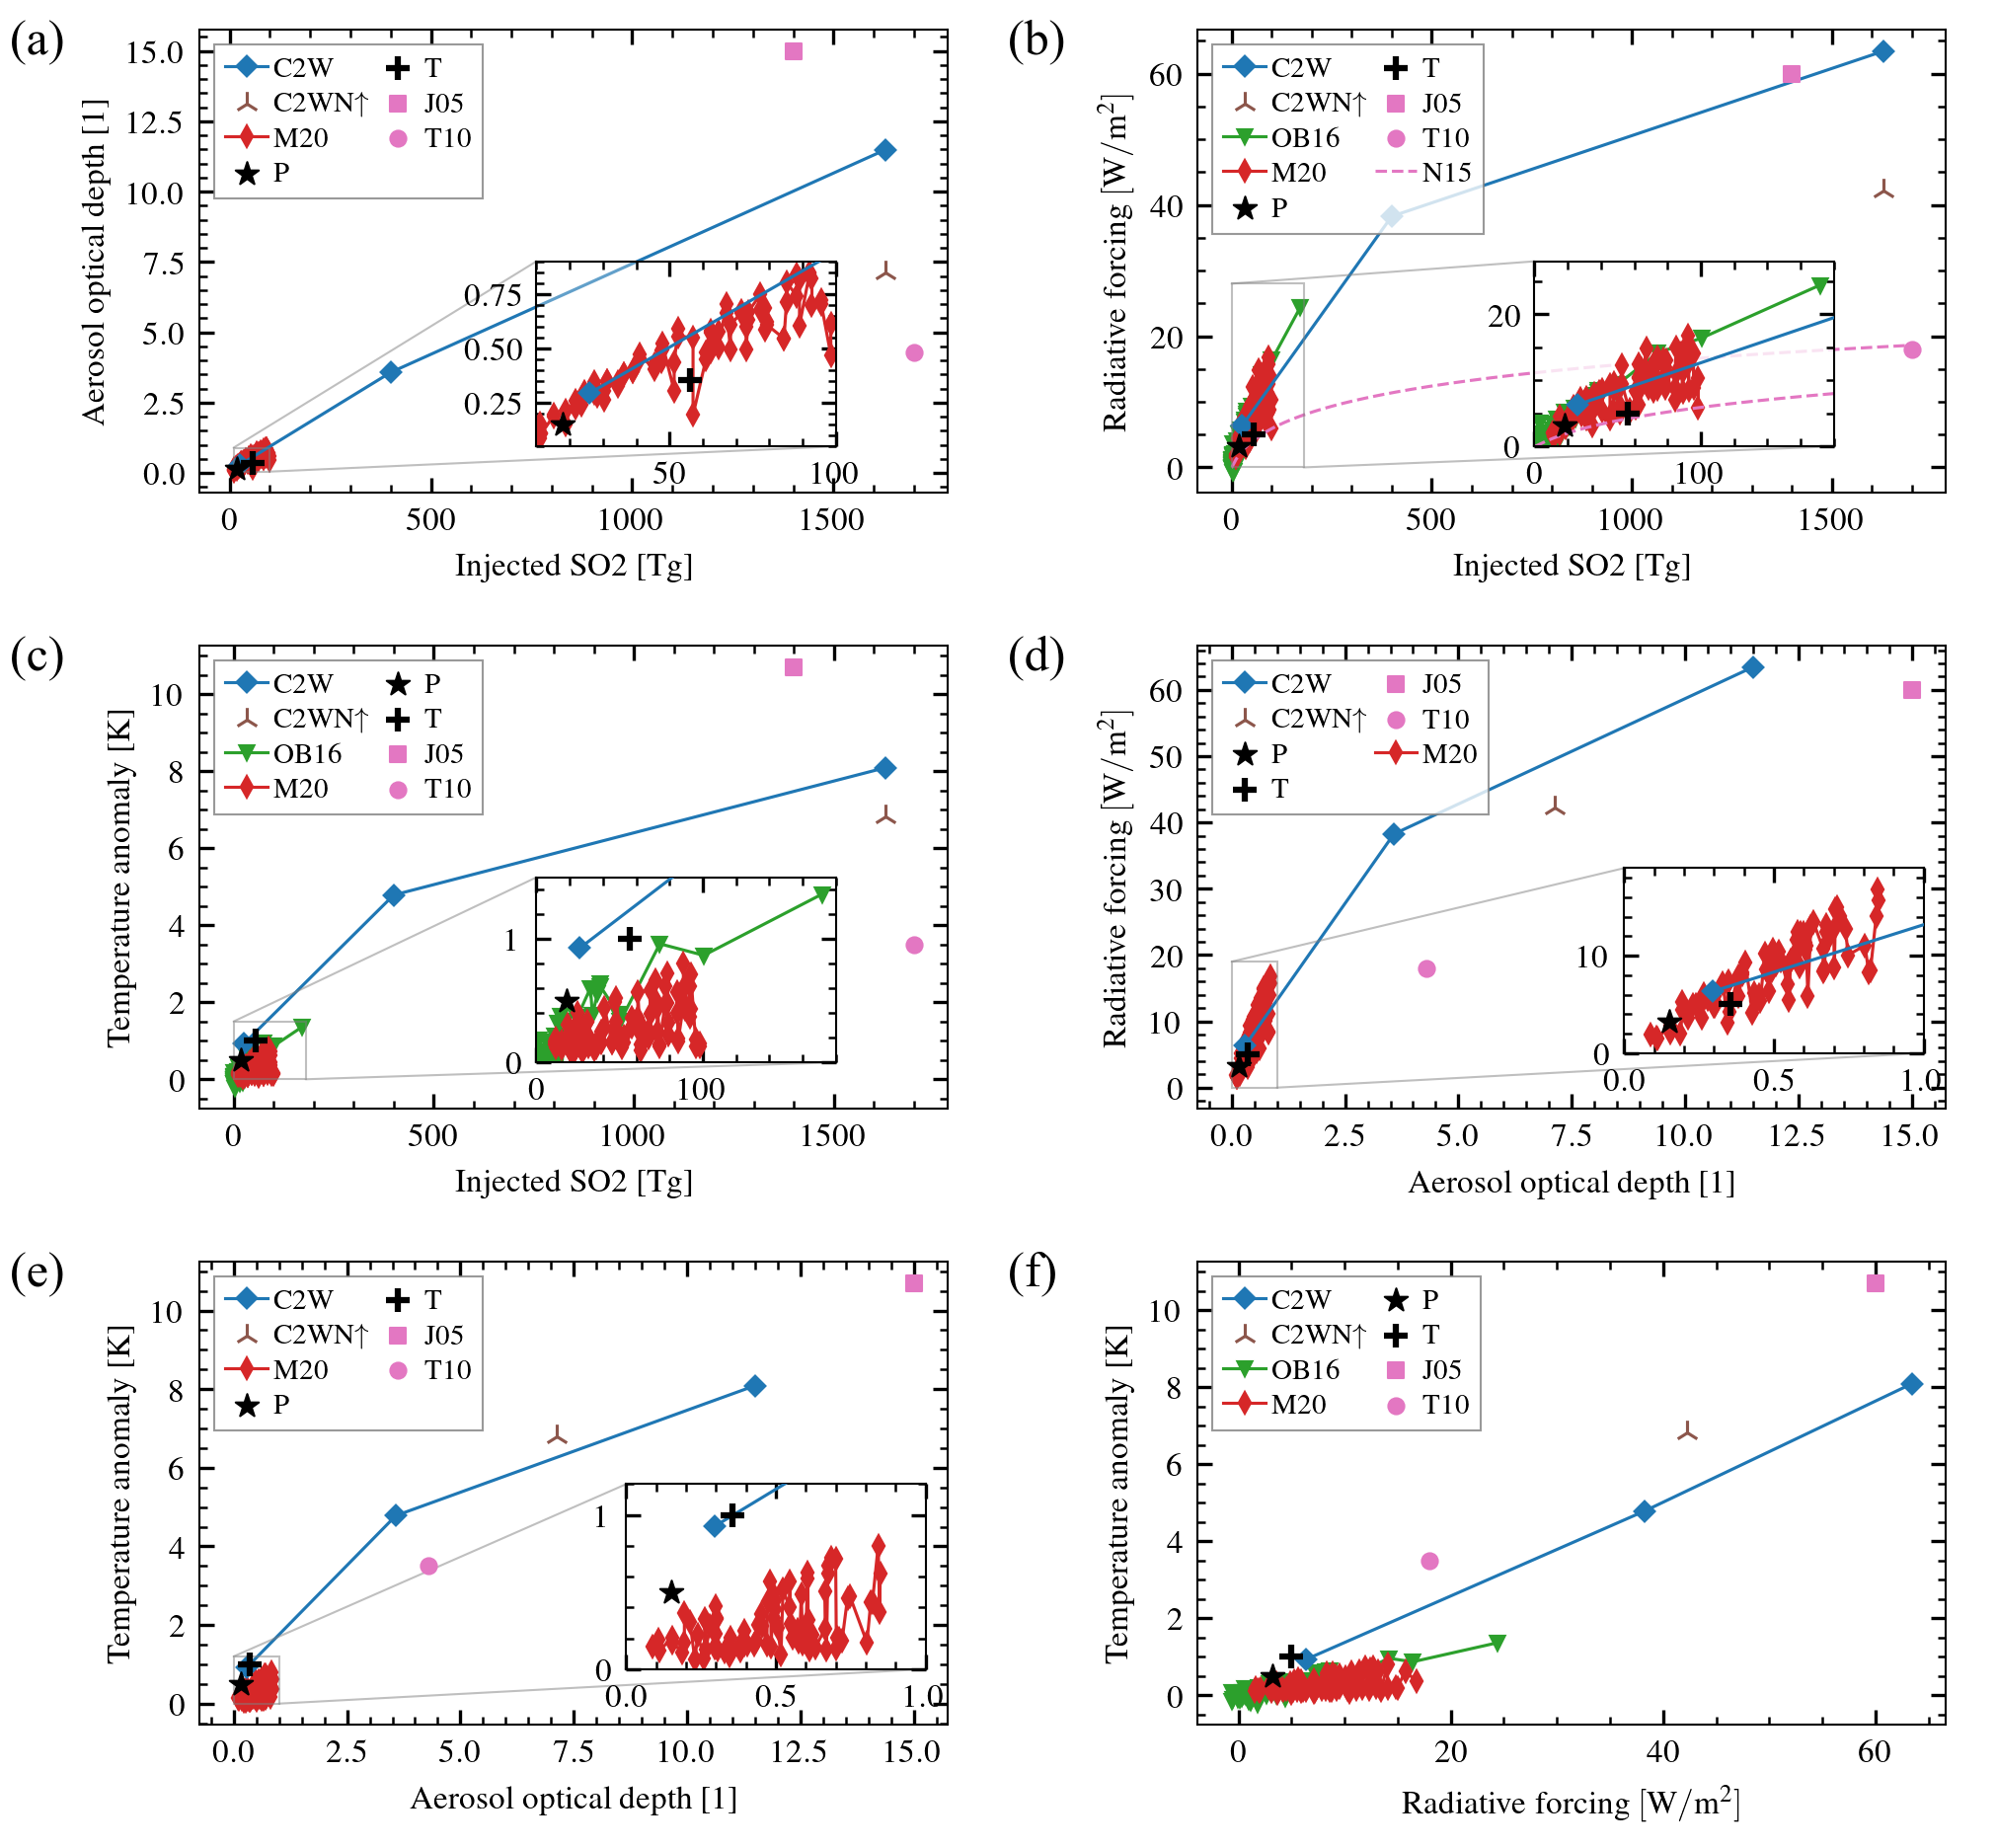
\includegraphics{figures/figure4.png}

  \caption{(a) \gls{aod} (b) \gls{rf} and (c) temperature as a function of \iso{}\@. (d)
    \gls{rf} and (e) temperature as a function of \gls{aod}. (f) Temperature as a function
    of \gls{rf}. Blue diamonds labelled \gls{c2w} represent tropical cases (\gls{c2wm},
    \gls{c2wmp}, \gls{c2ws}), the brown three-branched twig signifies the \gls{c2wsn} case,
    and green downward triangles denote \gls{ob16} data from \citet{ottobliesner2016}. The
    red thin diamonds labelled \gls{m20} display the \citet{marshall2020dataset} data.
    Purple star and yellow plus indicate Mt.\ Pinatubo and Mt.\ Tambora estimates based on
    observations. The pink square labelled \gls{j05} refers to the one-hundred times Mt.\
    Pinatubo super-volcano from \citet{jones2005}, and the pink disk labelled \gls{t10}
    represents the \gls{ytt} super-volcano from \citet{timmreck2010}. The pink dashed line
    labelled \gls{n15} is from \citet{niemeier2015}, indicating the function in
    eq.~\ref{eq:niemeier_exponential}.}\label{fig:parameter_scan}%
\end{figure*}

% INFO: the conversion between S and SO2 is confirmed by Niemeier and Timmreck (2015)'s
% reference to the Bekki et al. (1996) paper. Bekki uses 6000 Mt SO2, Niemeier uses 3000
% Tg(S).
\citet{niemeier2015} conducted simulations of continuous sulphur injections up to
\(\SI{200}{\tera\gram(\ce{SO2})\mathrm{yr}^{-1}}\) in the ECHAM5's middle atmosphere
version \citep{giorgetta2006} with aerosol microphysics from HAM \citep{stier2005}. They
observed an \gls{rf} dependence on injection rate \(x\) following an inverse exponential
converging to \(\SI{-65}{\watt\meter^{-2}}\) depicted in fig.~\ref{fig:parameter_scan}b
as the stippled pink line and given as

\begin{equation}
  \Delta
  R_{\mathrm{TOA}} =
  -\SI{65}{\watt\metre^{-2}}
  \mathrm{e}^{-{\left(\frac{\SI{2246}{\tera\gram(S)yr^{-1}}}{x}\right)}^{0.23}}.
  \label{eq:niemeier_exponential}
\end{equation}

Both our simulations and the findings from \citet{ottobliesner2016} exhibit a notably
slower increase than the exponential function. Interestingly, the simulations by
\citet{timmreck2010}, utilising the MPI-ESM and driven by \gls{aod} data from the HAM
aerosol model, for an eruption simulating the \gls{ytt} event
(\(\SI{850}{\tera\gram(\ce{S})}\)), closely correspond to the function presented in
eq.~\ref{eq:niemeier_exponential}. This alignment stems from using the same aerosol
microphysical model in both \citet{timmreck2010} and \citet{niemeier2015}, alongside
highly similar \glspl{esm}; the MPI-ESM is the precursor of ECHAM6, the subsequent
version update from ECHAM5 \citep{kuma2023}. Beginning with an initial input of
\(\SI{850}{\tera\gram(\ce{S})}\) (equivalent to \(\SI{1700}{\tera\gram(\ce{SO2})}\)),
their estimated \gls{aod} led to a peak \gls{rf} of \(\SI{-18}{\watt\metre^{-2}}\) (pink
filled circle in fig.~\ref{fig:parameter_scan}b, labelled \gls{t10}). Notably, the peak
values from the \gls{m20} dataset align neatly within the upper boundary from the
\gls{cesm} data (\gls{c2w} and \gls{ob16}) and the lower limit defined by
eq.~\ref{eq:niemeier_exponential}. Eruptions closer to the equator within the \gls{m20}
dataset correspond to data points near the upper limit, while eruptions at higher
latitudes yield weaker peak \gls{rf} values closer to the lower boundary. Crucially,
none of the eruption simulations violated the suggested upper threshold of
\(\SI{-65}{\watt\metre^{-2}}\) as defined in eq.~\ref{eq:niemeier_exponential}.

Figure~\ref{fig:parameter_scan}c illustrates the response of temperature against \iso{}.
Similar to fig.~\ref{fig:parameter_scan}b, the \gls{c2w} data deviates, indicating a
relatively weaker temperature response with increased \iso{} levels. Notably, the
\gls{ob16} dataset takes a different trajectory compared to the \gls{c2w} data,
showcasing less extreme temperature fluctuations as \iso{} rises. In contrast to our
findings, \gls{t10} demonstrates a considerably weaker temperature perturbation, noting
a maximum temperature anomaly of only \(\SI{-3.5}{\kelvin}\) for their
\(\SI{1700}{\tera\gram(\ce{SO2})}\) eruption, while \gls{j05} records a substantially
greater maximum temperature anomaly of \(\SI{-10.7}{\kelvin}\) compared to our \gls{c2w}
simulations.

Moving to fig.~\ref{fig:parameter_scan}d, we revisit the relationship between \gls{rf}
and \gls{aod}, focusing on peak values rather than annual and seasonal averages. As
previously discussed, the \gls{rf} to \gls{aod} ratio displays weaker alignment than
previous studies \citep{jones2005, marshall2020, timmreck2010}, with \gls{c2w} peak
values not conforming to a linear trend. This comparison suggests potential significant
dependencies on the model and its input parameters, such as latitude. These complexities
add to the noise, which for the relatively small ensemble size of four used here may be
significant.

For fig.~\ref{fig:parameter_scan}e, the \gls{c2w} data is anticipated to resemble the
patterns observed in fig.~\ref{fig:parameter_scan}c due to the nearly linear association
identified between \gls{aod} and \iso{} in fig.~\ref{fig:parameter_scan}a. Although the
relationship between temperature and \gls{aod} appears to follow a similar trend,
stronger conclusions would necessitate additional data. Notably, the parallels between
the \gls{m20} data in figs.~\ref{fig:parameter_scan}c and~\ref{fig:parameter_scan}e are
evident; however, it's essential to acknowledge that these were conducted with
prescribed sea surface temperatures, preventing the surface temperature from being fully
perturbed.

Finally, in fig.~\ref{fig:parameter_scan}f, we compare the temperature and \gls{rf}
responses. Both the \gls{c2w} and \gls{ob16} datasets showcase a near-linear
relationship between temperature and \gls{rf}. The \gls{c2w} data indicates a steeper
gradient, potentially implying stronger temperature perturbations compared to
\gls{ob16}. However, limited data overlap and differences in model complexities prevent
robust conclusions, especially considering the potential biases in the values from the
analysis of the \gls{ob16} data, as outlined in Appendix B. This, along with
considerable noise, make the results from the analysis of the \gls{ob16} data less
reliable.

\section{Discussion}\label{sec:discussion}

% NOTE: Suggested layout for the
% Discussion:
% - Explain the results and emphasize significant findings clearly
% - Discuss the impact and importance of results compared with recent relevant research
% Conclusion
% - The justification for these objectives: Why is the work important?
% - Summarize the key points made in the other sections
% - Conclude overall discussion of article
% - Link this section to the introduction

\subsection{Linearity between \gls{aod} and \gls{rf}}

Figures~\ref{fig:aod_vs_toa_ses_avg},~\ref{fig:aod_vs_toa_avg_loop_ratios} and
\ref{fig:parameter_scan}d collectively demonstrate that as the \gls{aod} surpasses
approximately \(1.0\), the scaling of approximately
\(\SI{-20}{\watt\metre^{-2}\mathrm{AOD}^{-1}}\) no longer corresponds to proportional
values of \gls{rf}. For the intermediate volcanic eruption (\gls{c2wmp}) at
\(\SI{400}{\tera\gram(\ce{SO2})}\), a mostly linear relationship between \gls{rf} and
\gls{aod} emerge, displaying a slope of roughly
\(\SI{-10}{\watt\metre^{-2}\mathrm{AOD}^{-1}}\). As for the largest eruption, an
\gls{rf} scaling of approximately \(\sim \SI{-5}{\watt\metre^{-2}\mathrm{AOD}^{-1}}\)
yields reasonable values. The almost linear relationship between \iso{} and \gls{aod} in
fig.~\ref{fig:parameter_scan}a indicates that larger eruptions injecting more \ce{SO2}
create larger aerosols, leading to less effective radiation scattering, thereby
influencing the \gls{rf} but not the \gls{aod} \citep{english2013, timmreck2010,
  timmreck2018}.

\citet{timmreck2010} highlights that for sufficiently large eruptions like Mt.\ Pinatubo
and \gls{ytt}, \ce{OH} radicals are not abundant enough, which limit \ce{SO2} oxidation.
The \gls{aod} peak in the \gls{ytt} simulation, occurring six months after Mt.\
Pinatubo's peak \citet{timmreck2010}, remains substantially lower in value compared to a
\(100\times\) scaling (refer to Fig.\ 1c in \citet{timmreck2010}). This observation
aligns with our findings, as illustrated in fig.~\ref{fig:compare-waveform-temp}a, where
smaller eruptions show an earlier \gls{aod} peak. While \citet{timmreck2010} reports a
peak \gls{rf} anomaly of \(\SI{-18}{\watt\metre^{-2}}\) occurring \(7\)--\(8\) months
post-eruption, \citet{jones2005} suggests a \(\SI{-60}{\watt\metre^{-2}}\) anomaly one
year later. The \gls{rf} peak preceding the \gls{aod} peak, approximately \(6\)--\(8\)
months post-eruption in \gls{cesm2} (see fig.~\ref{fig:compare-waveform-temp}b), though
smaller in magnitude in \citet{timmreck2010}, aligns well with both the functional fit
by \citet{niemeier2015} and the lower bounds from eruption simulations in
\citet{marshall2020}. Hence, the \gls{aod} time series appears influenced by \iso{}
magnitude, affecting the peak timing, while the \gls{rf} time series shows a similar
shape with reduced magnitudes as \iso{} increases.

Although \gls{j05} data is comparable to the \gls{c2ws} simulation concerning \gls{aod}
and \gls{rf}, the temperature response reported by \citet{jones2005} appears much
stronger than our most intense eruption. As \citet{jones2005} multiplies the \gls{aod}
forcing from Mt.\ Pinatubo by one hundred, the resulting time series significantly
deviates from a super-eruption scenario, potentially causing a substantially stronger
temperature perturbation. Additionally, \citet{timmreck2010}, using a more realistic
\gls{aod} forcing, observes much smaller cooling compared to \citet{jones2005}.

The biggest spread in the date is found when converting from \iso{} to any of the three
output parameters when comparing across models. Conversion from \iso{} to \gls{aod} is
consistent within similar models, even when comparing simulations of volcanic eruptions
\citep{timmreck2010} and continuous injection of \ce{SO2} \citep{niemeier2015}, but has
a wide spread at large values of \iso{} across model families
(figs.~\ref{fig:parameter_scan}a,b,c). Comparatively, the \gls{rf}
(fig.~\ref{fig:parameter_scan}d) and temperature (fig.~\ref{fig:parameter_scan}e) as a
function of \gls{aod} demonstrate a smaller spread across models, and consequently, the
spread for temperature as a function of \gls{rf} (fig.~\ref{fig:parameter_scan}f) is
also small. Previous studies assumed a roughly linear relationship between \gls{rf} and
\gls{aod}, particularly for lower values of \gls{aod} and \gls{rf}, where the estimated
slope was notably steeper at around \(\SI{-20}{\watt\metre^{-2}\mathrm{AOD}^{-1}}\) for
\(\mathrm{AOD}<1\) compared to the approximately
\(\SI{-5}{\watt\metre^{-2}\mathrm{AOD}^{-1}}\) observed here at \(\mathrm{AOD}\gg1\).
Hence, a linear relationship appears to be an accurate estimate of \gls{rf} dependence
on \gls{aod} for eruptions similar to or smaller than Mt.\ Pinatubo. However, for larger
eruptions, factors like \ce{OH} scarcity and aerosol growth, influencing reflectance and
their gravitational pull, substantially impact both \gls{aod} and \gls{rf} evolution.

Notably, from the \gls{c2w} cases, a post-eruption time dependency on the \gls{rf} to
\gls{aod} ratio emerges. \citet{marshall2020} discusses a similar aspect, noting that
while the efficiency increases from year 1 to year 2 when examining \gls{aod} and
\gls{rf}, here, the efficiency decreases over time, as depicted in
fig.~\ref{fig:aod_vs_toa_avg_loop_ratios}. This is by \citet{marshall2020} attributed to
the time taken for aerosol dispersion, affecting global albedo and consequently
\gls{rf}, whereas \gls{aod} is less affected by aerosol dispersion. Focusing solely on
tropical eruptions in \gls{m20} (between \(-10\) and \(\SI{10}{\degree\mathrm{N}}\)),
the \gls{rf} to \gls{aod} ratio closely resembles the findings from \gls{c2wmp}
simulations. Thus, while \iso{} is crucial for estimating the average time of the
\gls{rf} to \gls{aod} ratio, latitude and specifically aerosol dispersion seem more
influential in determining the post-eruption evolution of the ratio. Given that
\gls{c2wsn} cases lack a significant increase in ratio akin to tropical eruption
simulations (\gls{c2w}), the substantial difference in eruption latitude appears to be a
likely cause.

\citet{marshall2019, marshall2020, marshall2021} utilise a code with seven log-normal
modes to simulate aerosol mass and number concentrations, along with an atmosphere-only
configuration with prescribed sea surface temperatures and sea ice extent
\citep{marshall2019}. This approach contrasts with \gls{cesm2}, which operates as an
\gls{esm}. The configuration employed by \citet{marshall2019} is from the UM-UKCA model,
an extended version of HadGEM3 \citep{dhomse2014}, which belongs to a different model
family than both \gls{cesm2} and ECHAM5/MPI-ESM (utilised by \citet{timmreck2010,
  niemeier2015}) but shares an ancestry with HadCM3 (utilised by \citet{gregory2016})
\citep{kuma2023}, see Appendix C for a more detailed summary of the model families used.
Based on fig.~\ref{fig:parameter_scan}, the model family seems pivotal in determining
the estimated \gls{aod} and \gls{rf} magnitudes from \iso{}, whereas the various models
generally demonstrate more consistency in representing \gls{rf} from \gls{aod}. Given
that \gls{m20} employs a model from a distinct family compared to both \gls{ob16} and
\gls{c2w} cases, and \gls{t10} and \gls{n15}, while covering the parameter space between
the two families, it would be intriguing to include higher \iso{} values in the
\gls{m20} data to explore whether it remains bounded below (by \gls{t10} and \gls{n15})
and above (by \gls{ob16} and \gls{c2w}). This also prompts questions about whether
\iso{} saturation at a specific level, as illustrated in \citet{niemeier2015}, yields a
lower bound \gls{rf} efficiency estimate, similar to what a high-latitude eruption might
produce. Alternatively, differences in model aerosol chemistry might account for the
wide range in \gls{rf} as a function of \iso{}.

In summary, smaller eruptions and their estimates produce a relatively substantial
\gls{rf} to \gls{aod} ratio (\(\sim \SI{-20}{\watt\metre^{-2}\mathrm{AOD}^{-1}}\)),
whereas larger eruptions (or yearly \iso{} in the atmosphere as applied in
\citet{niemeier2015}) result in estimates with smaller magnitudes (\(\sim
\SI{-10}{\watt\metre^{-2}\mathrm{AOD}^{-1}}\) to \(\sim
\SI{-5}{\watt\metre^{-2}\mathrm{AOD}^{-1}}\), as depicted in
fig.~\ref{fig:aod_vs_toa_avg_loop_ratios}). \citet{niemeier2017} indicates a decrease in
efficiency as the injection rate increases, connected to larger volcanic eruptions
leading to larger aerosol particle sizes, thereby decreasing forcing efficiency per
\iso{} \citep{english2013, timmreck2018}.

\subsection{Climate sensitivity estimate}

As previously mentioned, the outcomes from \gls{j05} closely resemble our \gls{c2ws}
scenario concerning both \gls{aod} and \gls{rf} values, yet significantly differ in
temperature. To delve deeper into this discrepancy, we aim to conduct a comparison
between their reported climate feedback parameter \(\alpha \) (where \(s=1/\alpha \) is
the climate sensitivity parameter) with our estimations of climate resistance, denoted
as \(\rho \), and the \gls{tcrp} \(1/\rho\) (where \(\mathrm{TCS}=F_{2\times}\times
\mathrm{TCRP}\) is the transient climate sensitivity). Although volcanic eruption
forcing typically endures for about a year, a duration too brief for the timescales at
which \(F=\rho T\) remains valid \citep{gregory2016}, a workaround involves using a
time-integral form introduced by \citet{merlis2014}:

\begin{equation}
  \int_0^{\tau}F \mathrm{d}t=\rho\int_{0}^{\tau}T \mathrm{d}t
\end{equation}
\begin{equation}
  \rho=\frac{\int_0^{\tau}F \mathrm{d}t}{\int_{0}^{\tau}T \mathrm{d}t}.
  \label{eq:climate-resistance}
\end{equation}

If the upper bound of the integral, \(\tau \), is sufficiently large so that the upper
ocean heat capacity is the same at \(t=0\) and \(t=\tau \), this aligns with \(F=\rho
T\) \citep{gregory2016} (\citet{merlis2014} utilised \(\tau =\SI{15}{\mathrm{y}}\)).
Additionally, it's worth noting that the climate resistance and the climate feedback
parameter are associated with the ocean heat uptake efficiency (\(\kappa \)) through
\(\rho =\alpha +\kappa \).

The climate feedback parameter, as estimated by \citet{jones2005}, stands at
approximately \(\alpha \simeq \SI{4}{\watt\metre^{-2}\kelvin^{-1}}\), exceeding twice
the value obtained by \citet{gregory2016} in their simulations using Mt.\ Pinatubo
within the HadCM3 climate model.

We determine the climate resistance using the integral-form computation outlined in
eq.~\ref{eq:climate-resistance} and adopting \(\tau =\SI{8}{\mathrm{yr}}\), coinciding
with the duration of our simulations. The estimated climate resistance \(\rho \) from
the three tropical simulation cases (with four in each ensemble) yields
\(\num{3.3(9)}\), \(\num{3.12(9)}\), and \(\num{2.91(8)}\), and \gls{tcrp} (\(1/\rho\))
values of \(\num{0.32(7)}\), \(\num{0.321(9)}\), and \(\num{0.34(1)}\), as demonstrated
in table~\ref{tab:trcp}.

The climate resistance parameter \(\rho\) differs from the climate feedback parameter
estimated by \citet{jones2005} (\(\alpha\)). However, considering both \(\alpha \) and
\(\kappa \) are positive, and our calculated values of \(\rho (=\alpha +\kappa) \) are
all smaller than the \citet{jones2005} estimate of \(\alpha \simeq
\SI{4}{\watt\metre^{-2}\kelvin^{-1}}\), we deduce that the climate feedback parameter
linked to the simulations conducted here must be notably lower than what
\citet{jones2005} found. It is worth noting that the temperature time series are not
fully returned to equilibrium after eight years, which would add to the estimated values
of \(\rho \) from the time-integral, but it is expected that this contribution is small
compared to the estimates. Since the temperature perturbation obtained by \gls{j05} was
higher than any achieved here, it indicates that the forcing used by \gls{j05} must be
more potent. The primary contributor to this increased forcing strength is believed to
stem from the shape of the \gls{aod} time series utilised, rather than the magnitude, as
the magnitude was comparable to that used in the \gls{c2ws} and \gls{c2wsn} cases.

\begin{table}
  \centering

  \caption{Estimated climate resistance and \gls{tcrp} by use of the method outlined by
    \citet{merlis2014}. Estimates are based on ensembles with four members, and where \(\tau
    =\SI{8}{\mathrm{yr}}\) in eq.~\ref{eq:climate-resistance}}\label{tab:trcp}%
  \begin{tabular}{ccc}
    Simulation type & \(\rho [\si{\watt\metre^{-2}\kelvin^{-1}}]\) & \(1/\rho\)         \\
    \gls{c2ws}      & \(\num{2.91(8)}\)                            & \(\num{0.34(1)}\)  \\
    \gls{c2wmp}     & \(\num{3.12(9)}\)                            & \(\num{0.321(9)}\) \\
    \gls{c2wm}      & \(\num{3.3(9)}\)                             & \(\num{0.32(7)}\)  \\
  \end{tabular}
\end{table}

\section{Conclusions}\label{sec:conclusions}

In this paper we considered three large to super-volcano sized eruptions. We investigate
the \gls{rf} as a function of \gls{aod} and look at their ratio, and find that the
\gls{rf} dependence of \(\sim\SI{-20}{\watt\metre^{-2}\mathrm{AOD}^{-1}}\) is consistent
with our results for eruptions of similar size in terms of \iso{} as Mt.\ Pinatubo.
Larger eruptions with one to two orders of magnitude more \iso{} is found to produce a
much more shallow gradient closer to \(\sim
\SI{-5}{\watt\metre^{-2}\mathrm{AOD}^{-1}}\). A more shallow gradient for larger
eruptions is also consistent with data from previous studies of super-volcanoes.

We find that there is generally hard to find a consistent conversion between \iso{} and
\gls{aod} that translates well between models, while from our simulations in the
\gls{cesm2} there is close to a linear relationship between \iso{} and \gls{aod}.

The time-after-eruption dependence of the ratio between \gls{rf} and \gls{aod} have been
reported before, but where the efficiency increased with time \citep{marshall2020}, that
is, \gls{rf} became relatively larger when compared with \gls{aod}. Our simulations
rather show a decrease in the aerosol forcing efficiency, where the \gls{aod} was
relatively larger than \gls{rf} later in the eruption phase. We also find that the same
trend is indeed found in the \gls{m20} dataset when including only tropical eruptions,
and as such conclude that latitude is significant in deciding the aerosol forcing
efficiency generally, and as a function of time-after-eruption specifically.

An interesting aspect concerning the decay phase in both the \gls{aod} and the \gls{rf}
time series is the influence of the decay on the temperature time series, perhaps
inducing a trend. That is, do the temperature time series decay similarly to either the
\gls{aod} or the \gls{rf}? Allowing the simulations to run for at least twenty years to
enable the tail to be well resolved is therefore another avenue that could be explored
further.

\clearpage
%%%%%%%%%%%%%%%%%%%%%%%%%%%%%%%%%%%%%%%%%%%%%%%%%%%%%%%%%%%%%%%%%%%%%
% ACKNOWLEDGMENTS
%%%%%%%%%%%%%%%%%%%%%%%%%%%%%%%%%%%%%%%%%%%%%%%%%%%%%%%%%%%%%%%%%%%%%
\acknowledgments{}
%  Keep acknowledgments (note correct spelling: no ``e'' between the ``g'' and
% ``m'') as brief as possible. In general, acknowledge only direct help in
%  writing or research. Financial support (e.g., grant numbers) for the work done,
%  for an author, or for the laboratory where the work was performed must be
%  acknowledged here rather than as footnotes to the title or to an author's name.
%  Contribution numbers (if the work has been published by the author's institution
%  or organization) should be placed in the acknowledgments rather than as
%  footnotes to the title or to an author's name.

% https://www.sigma2.no/acknowledgements
The simulations were performed on resources provided by Sigma2 --- the National
Infrastructure for High Performance Computing and Data Storage in Norway.

%%%%%%%%%%%%%%%%%%%%%%%%%%%%%%%%%%%%%%%%%%%%%%%%%%%%%%%%%%%%%%%%%%%%%
% DATA AVAILABILITY STATEMENT
%%%%%%%%%%%%%%%%%%%%%%%%%%%%%%%%%%%%%%%%%%%%%%%%%%%%%%%%%%%%%%%%%%%%%
%
%
\datastatement{}
%  The data availability statement is where authors should describe how the data underlying
%  the findings within the article can be accessed and reused. Authors should attempt to
%  provide unrestricted access to all data and materials underlying reported findings.
%  If data access is restricted, authors must mention this in the statement. See
%  {http://www.ametsoc.org/PubsDataPolicy} for more info.

% https://documentation.sigma2.no/nird_archive/user-guide.html
Data generated directly from output fields of \gls{cesm2} are available at \emph{refer
  to Sigma2 archive}. Analysis scripts are available at
\url{https://github.com/engeir/paper1-code} and is published to
\url{https://zenodo.org/doi/10.5281/zenodo.10229427}. Source files used to generate
\gls{cesm2} input files are available at \emph{github repo}.

%%%%%%%%%%%%%%%%%%%%%%%%%%%%%%%%%%%%%%%%%%%%%%%%%%%%%%%%%%%%%%%%%%%%%
% APPENDIXES
% https://www.ametsoc.org/index.cfm/ams/publications/author-information/latex-author-info/documentation-for-ams-latex-template1/
%%%%%%%%%%%%%%%%%%%%%%%%%%%%%%%%%%%%%%%%%%%%%%%%%%%%%%%%%%%%%%%%%%%%%
%
%% If only one appendix, use

%\appendix

%% If more than one appendix, use \appendix[<letter>], e.g.,

%\appendix[A]

%% Appendix title is necessary! For appendix title:

%\appendixtitle{Title of Appendix}

%%% Appendix section numbering (note, skip \section and begin with \subsection)
%
% \subsection{First primary heading}

% \subsubsection{First secondary heading}

% \paragraph{First tertiary heading}

\appendix

\appendix[A]

\appendixtitle{Simulation set up and output}

Simulations were created using a modified version of the file
\url{http://svn.code.sf.net/p/codescripts/code/trunk/ncl/emission/createVolcEruptV3.ncl},
via a Python project developed on GitHub at
\url{https://github.com/engeir/volcano-cooking}. The project is also available from the
Python package manager PyPI\@. The program creates volcanoes with a given \ce{SO2}
amount that is injected over six
hours\footnote{\url{http://svn.code.sf.net/p/codescripts/code/trunk/ncl/emission/createVolcEruptV3.ncl}}
at a given latitude, longitude and altitude. All volcanic \ce{SO2} files are created by
setting the eruption details in a~.json file that is read to the
\texttt{volcano-cooking} CLI at a fixed version, making for a reproducible experiment
setup.

We are using the \texttt{BWma1850} component
setup\footnote{\url{https://docs.cesm.ucar.edu/models/cesm2/config/2.1.0/compsets.html}}
to run the \gls{cesm2}, and an accompanying \gls{fsst} simulation to obtain estimates of
the \gls{rf}. The \gls{fsst} simulation used is not from a standardised component setup
as of \gls{cesm2} (v2.1.3), but is instead specified in full.\footnote{\fssturl} They
differ in \texttt{CICE -> CICE\%PRES}, which is prescribed sea-ice,
\texttt{POP2\%ECO\%DEP -> DOCN\%DOM} which is from a dynamical ocean to a prescribed
data ocean and the wave component \texttt{WW3 -> SWAV} which is now a stub wave
component instead of the full \gls{ww3}.

\gls{rf} is calculated as the combined (\gls{sw} and \gls{lw}) all-sky \gls{toa} energy
imbalance, where the \gls{cesm2} provide the output variables \gls{fsnt} and \gls{flnt}.
Thus, \(\mathrm{RF_*}= \mathrm{FSNT} - \mathrm{FLNT}\), and taking the difference
between volcanic simulations and a control simulation gives the final estimate of
\gls{rf} (\(\mathrm{RF}=\mathrm{RF_{VOLC}}-\mathrm{RF_{CONTROL}}\))
\citep{marshall2020}. The output parameters that go into this estimate are from he
\gls{fsst} simulation, hence this outline specifically describe how to calculate
\gls{erf} as opposed to \gls{irf}, which instead is the difference between the \gls{erf}
and the sum of all rapid atmospheric adjustments \citep{marshall2020,smith2018}. The
\gls{aod} is obtained from the output variable \gls{aodm}, while global temperature is
saved by \gls{cesm2} to the variable \gls{trefht}. These four output variables are all
that are used throughout this paper. The important input data used in the model
simulations are \iso{} in units of teragrams (\(\si{\tera\gram(\ce{SO2})}\)), used to
simulate volcanic eruptions.

\appendix[B]

\appendixtitle{Otto-Bliesner data analysis}\label{ap:ob16}

Data from \citet{ottobliesner2016} are the original input data of \iso{} as used in
their model simulations, where corresponding \gls{rf} and temperature data are found as
the value of the time series at the time of an eruption (according to the \iso{} time
series). Therefore, \gls{rf} and temperature values may be somewhat smaller in
figs.~\ref{fig:parameter_scan}b,c,f than their true value. Specifically, an ensemble of
5 is used for both \gls{rf} and temperature, and a mean from the 5 is used as the de
facto \gls{rf} and temperature time series. A control simulation of a single time series
is used to remove seasonal dependence from the temperature, where the control simulation
is averaged into a climatology mean. Further, a drift in the temperature is removed by
subtracting a linear regression fit. \gls{rf} have seasonality removed in the Fourier
domain. The forcing (\ce{SO2}) can be downloaded with direct link
\url{https://svn-ccsm-inputdata.cgd.ucar.edu/trunk/inputdata/atm/cam/volc/IVI2LoadingLatHeight501-2000_L18_c20100518.nc},
or found at \url{https://www.cesm.ucar.edu/working-groups/paleo/simulations/ccsm4-lm}
and \url{https://svn-ccsm-inputdata.cgd.ucar.edu/trunk/inputdata/atm/cam/volc/}.

The time of an eruption is decided based on a best attempt at aligning the \ce{SO2} time
series with both the \gls{rf} time series and the temperature time series individually.
The \gls{rf} and temperature values used in the \gls{ob16} data points are the exact
values at day 340 (\gls{rf}) and 400 (temperature) after the eruption according to the
\iso{} time series. Thus, missing the peak means the estimates will be biased towards
lower values, while other eruptions occurring close in time will contribute a bias to
higher values.

\appendix[C]

\appendixtitle{Model families}

The model utilised here was the \gls{cesm2} which is an ancestor of \gls{cesm1} utilised
by \gls{ob16}. They belong to a different model family than both the HadCM3 (\gls{j05}
and \gls{g16}) and the UM-UKCA (\gls{m20}), which is an extended version of HadGEM3
\citep{dhomse2014}, and an ancestor of HadCM3. A third model family is represented
through ECHAM5 (\gls{n15}) and MPI-ESM (\gls{t10}), where the latter is related to the
former via the ECHAM6. A summary of the model code genealogy is detailed in
table~\ref{tab:model-family}, based on the model code genealogy map created by
\citet{kuma2023}.

\begin{table*}
  \centering
  \caption{Model families and to which the different studies referred to in this paper
    reside. Based on the model code genealogy map by \citet{kuma2023}.}\label{tab:model-family}

  \begin{tabular}{ccc}
    Family relation                                                         & Model name           & Data point \\
    \multirow{2}{*}{CESM1 \(\rightarrow\) CESM1-CAM5 \(\rightarrow\) CESM2} & CESM1                & \gls{ob16} \\
                                                                            & CESM2
                                                                            & \emph{This
    contribution}                                                                                               \\
    \rowcolor{LightGray}                                                    & HadCM3
                                                                            & \gls{j05}, \gls{g16}              \\
    \rowcolor{LightGray}\multirow{-2}{*}{\shortstack{HadCM3 \(\rightarrow\) HadGEM1
    \(\rightarrow\)                                                                                             \\
    HadGEM2 \(\rightarrow\) HadGEM3 \(\rightarrow\) UM-UKCA}}               & UM-UKCA              &
    \gls{m20}                                                                                                   \\
    \multirow{2}{*}{ECHAM5 \(\rightarrow\) ECHAM6 \(\rightarrow\) MPI-ESM}  & ECHAM5               &
    \gls{n15}                                                                                                   \\
                                                                            & MPI-ESM              & \gls{t10}  \\
  \end{tabular}
\end{table*}

%%%%%%%%%%%%%%%%%%%%%%%%%%%%%%%%%%%%%%%%%%%%%%%%%%%%%%%%%%%%%%%%%%%%%
% REFERENCES
%%%%%%%%%%%%%%%%%%%%%%%%%%%%%%%%%%%%%%%%%%%%%%%%%%%%%%%%%%%%%%%%%%%%%
% Make your BibTeX bibliography by using these commands:
% \bibliographystyle{ametsocV6}
% \bibliography{references}

\bibliographystyle{ametsocV6} \bibliography{references} \clearpage
\printglossary[type=\acronymtype,title=List of Acronyms]

\end{document}
